% LuaLaTeX

\documentclass[a4paper, twoside, 12pt]{article}
\usepackage[latin]{babel}
%\usepackage[landscape, left=3cm, right=1.5cm, top=2cm, bottom=1cm]{geometry} % okraje stranky
\usepackage[landscape, a4paper, mag=1166, truedimen, left=2cm, right=1.5cm, top=1.6cm, bottom=0.8cm]{geometry} % okraje stranky

\usepackage{fontspec}
\setmainfont[Ligatures={Common, TeX}]{Junicode}
%\setmainfont{Junicode}

% shortcut for Junicode without ligatures (for the Czech texts)
\newfontfamily\nlfont[Ligatures={Common, TeX}]{Junicode}

% Hebrew font: http://scripts.sil.org/cms/scripts/page.php?site_id=nrsi&id=SILHebrUnic2
\newfontfamily\hebfont[Scale=1]{Ezra SIL}

\usepackage{multicol}
\usepackage{color}
\usepackage{lettrine}
\usepackage{fancyhdr}

% usual packages loading:
\usepackage{luatextra}
\usepackage{graphicx} % support the \includegraphics command and options
\usepackage{gregoriotex} % for gregorio score inclusion
\usepackage{gregoriosyms}
\usepackage{wrapfig} % figures wrapped by the text
\usepackage{parcolumns}
\usepackage[contents={},opacity=1,scale=1,color=black]{background}
\usepackage{tikzpagenodes}
\usepackage{calc}
\usepackage{longtable}
\usetikzlibrary{calc}

\setlength{\headheight}{14.5pt}

% Commands used to produce a typical "Conventus" booklet

\newenvironment{titulusOfficii}{\begin{center}}{\end{center}}
\newcommand{\dies}[1]{#1

}
\newcommand{\nomenFesti}[1]{\textbf{\Large #1}

}
\newcommand{\celebratio}[1]{#1

}

\newcommand{\hora}[1]{%
\vspace{0.5cm}{\large \textbf{#1}}

\fancyhead[LE]{\thepage\ / #1}
\fancyhead[RO]{#1 / \thepage}
\addcontentsline{toc}{subsection}{#1}
}

% larger unit than a hora
\newcommand{\divisio}[1]{%
\begin{center}
{\Large \textsc{#1}}
\end{center}
\fancyhead[CO,CE]{#1}
\addcontentsline{toc}{section}{#1}
}

% a part of a hora, larger than pars
\newcommand{\subhora}[1]{
\begin{center}
{\large \textit{#1}}
\end{center}
%\fancyhead[CO,CE]{#1}
\addcontentsline{toc}{subsubsection}{#1}
}

% rubricated inline text
\newcommand{\rubricatum}[1]{\textit{#1}}

% standalone rubric
\newcommand{\rubrica}[1]{\vspace{3mm}\rubricatum{#1}}

\newcommand{\notitia}[1]{\textcolor{red}{#1}}

\newcommand{\scriptura}[1]{\hfill \small\textit{#1}}

\newcommand{\translatioCantus}[1]{\vspace{1mm}%
{\noindent\footnotesize \nlfont{#1}}}

% pruznejsi varianta nasledujiciho - umoznuje nastavit sirku sloupce
% s prekladem
\newcommand{\psalmusEtTranslatioB}[3]{
  \vspace{0.5cm}
  \begin{parcolumns}[colwidths={2=#3}, nofirstindent=true]{2}
    \colchunk{
      \input{#1}
    }

    \colchunk{
      \vspace{-0.5cm}
      {\footnotesize \nlfont
        \input{#2}
      }
    }
  \end{parcolumns}
}

\newcommand{\psalmusEtTranslatio}[2]{
  \psalmusEtTranslatioB{#1}{#2}{8.5cm}
}


\newcommand{\canticumMagnificatEtTranslatio}[1]{
  \psalmusEtTranslatioB{#1}{temporalia/extra-adventum-vespers/magnificat-boh.tex}{12cm}
}
\newcommand{\canticumBenedictusEtTranslatio}[1]{
  \psalmusEtTranslatioB{#1}{temporalia/extra-adventum-laudes/benedictus-boh.tex}{10.5cm}
}

% volne misto nad antifonami, kam si zpevaci dokresli neumy
\newcommand{\hicSuntNeumae}{\vspace{0.5cm}}

% prepinani mista mezi notovymi osnovami: pro neumovane a neneumovane zpevy
\newcommand{\cantusCumNeumis}{
  \setgrefactor{17}
  \global\advance\grespaceabovelines by 5mm%
}
\newcommand{\cantusSineNeumas}{
  \setgrefactor{17}
  \global\advance\grespaceabovelines by -5mm%
}

% znaky k umisteni nad inicialu zpevu
\newcommand{\superInitialam}[1]{\gresetfirstlineaboveinitial{\small {\textbf{#1}}}{\small {\textbf{#1}}}}

% pars officii, i.e. "oratio", ...
\newcommand{\pars}[1]{\textbf{#1}}

\newenvironment{psalmus}{
  \setlength{\parindent}{0pt}
  \setlength{\parskip}{5pt}
}{
  \setlength{\parindent}{10pt}
  \setlength{\parskip}{10pt}
}

%%%% Prejmenovat na latinske:
\newcommand{\nadpisZalmu}[1]{
  \hspace{2cm}\textbf{#1}\vspace{2mm}%
  \nopagebreak%

}

% mode, score, translation
\newcommand{\antiphona}[3]{%
\hicSuntNeumae
\superInitialam{#1}
\includescore{#2}

#3
}
 % Often used macros
%%%% Preklady jednotlivych zpevu (nektere se opakuji, a je dobre mit je
% vsechny na jedne hromade)

\newcommand{\trOratioAnteOfficium}{\translatioCantus{Otevři, Pane, má ústa, abych chválil tvé svaté jméno.
Očisti mé srdce od všech marnivých, zvrácených a~jiných myšlenek, osvěť rozum, rozněť cit,
abych mohl důstojně, soustředěně a~zbožně recitovat a~vysloužil si být
vyslyšen před tváří tvé velebnosti. Skrze Krista…}}

\newcommand{\trOratioPostOfficium}{\translatioCantus{\textit{Následující modlitbu
opatřil pro ty, kdo ji zbožně vyřknou po hodinkách, zesnulý papež Lev X.
odpustky za hříchy vzniklé při konání hodinek z~lidské křehkosti. Říká se
vkleče.}
Svatosvaté a~nerozdílné Trojici, ukřižovanému lidství našeho Pána Ježíše
Krista, přeblažené a~přeslavné plodné neporušenosti vždy Panny Marie
i~souhrnu všech svatých buď ode všeho stvoření věčná chvála, čest a~sláva, nám
pak buď dáno odpuštění všech hříchů, po nekonečné věky věků. Amen.}}

% HOURS ---

\newcommand{\trAntI}{\translatioCantus{Jasné narození slavné Panny Marie,
z pokolení (dosl. ze semene) Abrahámova, vzešlé z kmene Judova, z rodu Davidova.}}
\newcommand{\trAntII}{\translatioCantus{Dnes je Narození svaté Panny 
Marie, jejíž předrahý život osvěcuje všechny církve.}}

\newcommand{\trAntIII}{\translatioCantus{Maria, jež vzešla 
z královského rodu, září; myslí i duchem ji zbožně prosíme, aby 
nám pomáhala svými přímluvami.}}

\newcommand{\trAntIV}{\translatioCantus{Srdcem i duchem pějme Kristu 
k slávě o této svaté slavnosti vznešené Rodičky Boží Marie.}}

\newcommand{\trAntV}{\translatioCantus{Příjemně \notitia{?} 
oslavujme Narození blahoslavené Marie,
aby se ona za nás přimlouvala u Pána Ježíše Krista.}}

\newcommand{\trCapituli}{\translatioCantus{Před věky, na počátku mě stvořil, potrvám věčně. Ve svatém Stanu jsem před ním konala službu.}}

\newcommand{\trRespVesp}{\translatioCantus{Buď zdráva, Maria,
plná milosti: \grestar{} Pán s tebou. \Vbardot{} Požehnaná jsi mezi ženami,
a požehnaný plod života (ve smyslu lůna, břicha) tvého.}}

\newcommand{\trVersus}{\translatioCantus{\Vbardot{} Dnes je Narození svaté Panny Marie. \Rbardot{} Jejíž předrahý život osvěcuje všechny církve.}}

\newcommand{\trAntMagnificatI}{\translatioCantus{Konejme památku
veledůstojného narození slavné Panny Marie,
jíž se dostalo mateřské důstojnosti bez ztráty panenské cudnosti.}}

% Tento preklad je vice nez nejisty a ani alternativy, ktere jsem
% videl, me nepresvedcily...
\newcommand{\trAntBenedictus}{\translatioCantus{Slavnostně slavme 
dnešní narození Marie, vždy Panny a Rodičky Boží: v něm se objevuje
vysokost trůnu (totiž Marie, trůnu Božího Syna), aleluja.}}

\newcommand{\trAntMagnificatII}{\translatioCantus{Tvé narození,
Bohorodičko Panno, vyhlásilo radost celému světu:
z tebe totiž vzešlo Slunce spravedlnosti, Kristus, náš Bůh:
jenž zrušil kletbu a dal nám požehnání: přemohl smrt a dal nám život věčný.}}

\newcommand{\trOrationis}{\translatioCantus{Prosíme tě, Bože, 
uděl svým služebníkům dar nebeské milosti,
aby těm, jimž slehnutím blahoslavené Panny vyvstal počátek spásy, 
slavnost k poctě jejího narození přinesla
rozhojnění pokoje.
Skrze tvého Syna, našeho Pána Ježíše Krista, který s tebou žije a kraluje,
Bůh, v jednotě Ducha svatého po všechny věky věků.}}

\newcommand{\trFideliumAnimae}{\translatioCantus{\Vbardot{} Duše věrných ať pro
milosrdenství Boží odpočívají v~pokoji. \Rbardot{} Amen.}}

% Completorium

\newcommand{\trJubeDomne}{\translatioCantus{Rač, pane, požehnat.}}

\newcommand{\trComplBenedictio}{\translatioCantus{Pokojnou noc a~svatou smrt
nechť nám dopřeje všemohoucí Pán. \Rbardot{} Amen.}}

\newcommand{\trComplLectioBr}{\translatioCantus{Buďte střízliví, bděte.
Váš protivník Ďábel obchází jako lev řvoucí a~hledá, koho by pohltil.
Postavte se proti němu pevní ve víře.  Ale ty, Pane, smiluj se nad námi.
\Rbardot{} Bohu díky.}}

\newcommand{\trComplAntI}{\translatioCantus{Rač se smilovati nade mnou,
Hospodine, a vyslyš mou modlitbu.}}

\newcommand{\trComplCapituli}{\translatioCantus{Jsi přece, Hospodine,
uprostřed nás a~jmenujeme se po tobě.  Neopouštěj nás, Pane, náš Bože.}}

\newcommand{\trRespCompl}{\translatioCantus{Do tvých rukou, Pane, \grestar{}
poroučím svého ducha. \Vbardot{} Ty mne zachráníš, Pane, Bože věrný.}}

\newcommand{\trComplVersus}{\translatioCantus{\Vbardot{} Střez mne jako zřítelnici oka,
aleluja. \Rbardot{} Ve stínu svých křídel uschovej mne, aleluja.}}

\newcommand{\trAntSalvaNos}{\translatioCantus{Ochraňuj nás, Pane, když
bdíme, a~buď s~námi, když spíme, ať bdíme s~Kristem a~odpočíváme v~pokoji.}}

\newcommand{\trComplOrationis}{\translatioCantus{Zavítej, prosíme, Pane, sem
do našeho příbytku a~daleko od něj zažeň všechny úklady nepřítele. Ať tu
bydlí tví svatí andělé a~tvoje požehnání buď nad ním stále. Skrze…}}

\newcommand{\trSalveRegina}{\translatioCantus{Zdrávas Královno, matko
milosrdenství, živote, sladkosti a naděje naše, buď zdráva!
K tobě voláme, vyhnaní synové Evy,
k tobě vzdycháme, lkajíce a plačíce
v tomto slzavém údolí.
A proto, orodovnice naše,
obrať k nám své milosrdné oči
a Ježíše, požehnaný plod života svého,
nám po tomto putování ukaž,
ó milostivá, ó přívětivá,
ó přesladká, Panno Maria!}}

\newcommand{\trOraProNobis}{\translatioCantus{\Vbardot{} 
Oroduj za nás, svatá Boží Rodičko,
\Rbardot{} aby nám Kristus dal účast na svých zaslíbeních.}}

% Matutinum

\newcommand{\trMatInvitatorium}{\translatioCantus{}}

\newcommand{\trMatVeniteA}{\translatioCantus{Pojďte, chvalme s~radostí Pána,
s~jásotem slavme Boha, svou spásu; předstupme před tvář jeho s~díky, písně plesu pějme jemu.}}

\newcommand{\trMatVeniteB}{\translatioCantus{Neboť Bůh veliký jest Hospodin, a~král nade všecky bohy.
Jsouť v~jeho ruce všecky hlubiny země, temena hor jsou majetek jeho.}}

\newcommand{\trMatVeniteC}{\translatioCantus{Jehoť jest moře, neb on je učinil; i~souš
je dílo jeho rukou. Pojďme, klanějme se, padněme, klekněme před Pánem, svým
tvůrcem. Jeť on Pán, náš Bůh, a~my jsme lid, jejž on vodí a~ovce, jež pase.}}

\newcommand{\trMatVeniteD}{\translatioCantus{Kéž byste poslechli dnes hlasu jeho:
,,Nezatvrzujte svých srdcí jak v~Hádce, jak v~Pokušení na poušti, kde vaši otcové pokoušeli mne,
zkoušeli mne, ač vídali skutky mé.``}}

\newcommand{\trMatVeniteE}{\translatioCantus{Čtyřicet roků mrzel jsem se na to pokolení
a~řekl jsem: ,,Lid je to myslí stále bloudící``! Oni však nechtěli znáti mé cesty, takže jsem
přisáhl ve svém hněvu: ,,Nedojdou odpočinku mého!\mbox{}``}}

\newcommand{\trMatAntI}{\translatioCantus{}}

\newcommand{\trMatAntII}{\translatioCantus{}}

\newcommand{\trMatAntIII}{\translatioCantus{}}

\newcommand{\trMatVersusI}{\translatioCantus{}}

\newcommand{\trMatAbsolutioI}{\translatioCantus{Vyslyš Pane Ježíši Kriste
prosby svých služebníků \gredagger{} a~smiluj se nad námi, \grestar{} jenž
s~Otcem a~Duchem…}}

\newcommand{\trMatBenedictioI}{\translatioCantus{Rač, pane, požehnat.
Věčný Otec nám stále žehnej. \Rbardot{} Amen.}}

\newcommand{\trMatLecI}{\translatioCantus{Kéž by mě zulíbal polibky svých úst. 
Tvé milování je nad víno lahodnější;
vybraně voní tvé voňavky;
rozlévající se olej je tvé jméno,
proto tě dívky milují.
Strhni mě za sebou, poběžme!
Král mě uvedl do svých komnat;
budeš nám radostí a jásotem.
Víc než víno oslavíme tvé milování;
věru po právu jsi milován!
Snědá jsem, a přece krásná, jeruzalémské dcery,
jako stany kedarské,
jako šalmské závěsy.
}}

\newcommand{\trMatRespI}{\translatioCantus{}}

\newcommand{\trMatBenedictioII}{\translatioCantus{Rač, pane, požehnat.
Jednorozený Boží Syn nám žehnej \grestar{} a nám pomáhej. \Rbardot{} Amen.}}

\newcommand{\trMatLecII}{\translatioCantus{Nehleďte na mou osmahlou pleť:
to mě slunce ožehlo.
Synové mé matky se na mne rozzlobili,
poslali mě hlídat vinice.
A svou vinici, tu jsem nehlídala!
Pověz mi tedy, ty, jehož miluje mé srdce:
kam zavedeš své stádo pást,
kde ho necháš za poledne odpočívat?
Abych už nebloudila jako tulačka
poblíž stád druhů tvých.
Nevíš-li to, nejrásnější z žen,
jdi po stopách stáda
a kůzlata svá zaveď, ať se pasou
poblíž obydlí pastýřů.
Ke své klisně zapřažené do vozu faraonova
tebe, mé milá, přirovnávám.
Stále krásné jsou tvé líce s náušnicemi
i tvé hrdlo v náhrdelnících.}}

\newcommand{\trMatRespII}{\translatioCantus{}}

\newcommand{\trMatBenedictioIII}{\translatioCantus{Rač, pane, požehnat.
Milost Ducha Svatého ať osvítí nám smysly \grestar{} i srdce. \Rbardot{} Amen.}}

\newcommand{\trMatLecIII}{\translatioCantus{Zhotovíme ti zlaté náušnice
a kuličky ze stříbra.
Když král stoluje,
vydechuje můj nard svou vůni.
Můj milý je polštářek s myrhou,
jenž mi odpočívá mezi ňadry.
Můj milý je hrozen šáchoru
ve vinicích v Engadi.
Jak jsi krásná, milá moje,
jak jsi krásná!
Tvé oči jsou holubice.
Jak jsi krásný, můj milý,
jak líbezný!
Naše lože je samá zeleň.
Trámoví našeho domu je z cedru,
naše ostění z cypřiše.}}

\newcommand{\trMatRespIII}{\translatioCantus{}}

\newcommand{\trMatAntIV}{\translatioCantus{}}

\newcommand{\trMatAntV}{\translatioCantus{}}

\newcommand{\trMatAntVI}{\translatioCantus{}}

\newcommand{\trMatVersusII}{\translatioCantus{}}

\newcommand{\trMatAbsolutioII}{\translatioCantus{
Tvá milost a laskavost nechť nám pomáhá, jenž žiješ a vládneš s Otcem a Svatým Duchem na věky věků.}}

\newcommand{\trMatBenedictioIV}{\translatioCantus{Rač, pane, požehnat.
Bůh Otec všemohoucí, \grestar{} buď k nám milostivý a odpouštějící. \Rbardot{} Amen.}}

\newcommand{\trMatLecIV}{\translatioCantus{}}

\newcommand{\trMatRespIV}{\translatioCantus{}}

\newcommand{\trMatBenedictioV}{\translatioCantus{}}

\newcommand{\trMatLecV}{\translatioCantus{}}

\newcommand{\trMatRespV}{\translatioCantus{}}

\newcommand{\trMatBenedictioVI}{\translatioCantus{Rač, pane, požehnat.
Bůh rozněť v nás oheň své lásky. \Rbardot{} Amen.}}

\newcommand{\trMatLecVI}{\translatioCantus{}}

\newcommand{\trMatRespVI}{\translatioCantus{}}

\newcommand{\trMatAntVII}{\translatioCantus{}}

\newcommand{\trMatAntVIII}{\translatioCantus{}}

\newcommand{\trMatAntIX}{\translatioCantus{}}

\newcommand{\trMatVersusIII}{\translatioCantus{}}

\newcommand{\trMatAbsolutioIII}{\translatioCantus{Z okovů našich hříchů,
\grestar{} vysvoboď nás všemohoucí a milosrdný Pán. \Rbardot{} Amen.}}

\newcommand{\trMatBenedictioVII}{\translatioCantus{Rač, pane, požehnat.
Čtení evangelia nechť je nám \grestar{} spásou a ochranou. \Rbardot{} Amen.}}

\newcommand{\trMatLecVIIa}{\translatioCantus{
  Rodokmen Ježíše Krista, syna Davidova, syna Abrahámova:
  Abrahám zplodil Izáka,
  Izák zplodil Jakuba.}}

\newcommand{\trMatLecVIIb}{\translatioCantus{}}

\newcommand{\trMatRespVII}{\translatioCantus{}}

\newcommand{\trMatBenedictioVIII}{\translatioCantus{Rač, pane, požehnat.
\Rbardot{} Amen.}}

\newcommand{\trMatLecVIII}{\translatioCantus{}}

\newcommand{\trMatRespVIII}{\translatioCantus{}}

\newcommand{\trMatBenedictioIX}{\translatioCantus{Rač, pane, požehnat.
Do společnosti občanů nebes \grestar{} ať nás dovede král andělů.
\Rbardot{} Amen.}}

\newcommand{\trMatLecIX}{\translatioCantus{}}

% from the Czech Liturgia horarum
\newcommand{\trTeDeum}{\begin{translatioMulticol}{3}

Bože, tebe chválíme, 
tebe, Pane, velebíme.

Tebe, věčný Otče, 
oslavuje celá země.

Všichni andělé, 
cherubové i~serafové,

všechny mocné nebeské zástupy 
bez ustání volají:

Svatý, Svatý, Svatý, 
Pán, Bůh zástupů.

Plná jsou nebesa i~země 
tvé vznešené slávy.

Oslavuje tě 
sbor tvých apoštolů,

chválí tě 
velký počet proroků,

vydává o~tobě svědectví 
zástup mučedníků;

a~po celém světě 
vyznává tě tvá církev:

neskonale velebný, 
všemohoucí Otče,

úctyhodný Synu Boží, 
pravý a~jediný,

božský Utěšiteli, 
Duchu svatý.

Kriste, Králi slávy, 
tys od věků Syn Boha Otce;

abys člověka vykoupil, 
stal ses člověkem a~narodil ses z~Panny;

zlomil jsi osten smrti 
a~otevřel věřícím nebe;

sedíš po Otcově pravici 
a~máš účast na jeho slávě.

Věříme, že přijdeš soudit, 

a~proto tě prosíme:
přispěj na pomoc svým služebníkům, 
vždyť jsi je vykoupil svou předrahou krví;

dej, ať se radují s~tvými svatými 
ve věčné slávě.

Zachraň, Pane, svůj lid, žehnej svému dědictví, 
veď ho a~stále pozvedej.

Každý den tě budeme velebit 
a~chválit tvé jméno po všechny věky.

Pomáhej nám i~dnes, 
ať se nedostaneme do područí hříchu.

Smiluj se nad námi, Pane, 
smiluj se nad námi.

Ať spočine na nás tvé milosrdenství, 
jak doufáme v~tebe.

Pane, k~tobě se utíkáme, 
ať nejsme zahanbeni na věky. 
\end{translatioMulticol}}

\newcommand{\trMatEvangelium}{\translatioCantus{
  Rodokmen Ježíše Krista, syna Davidova, syna Abrahámova:
  Abrahám zplodil Izáka,
  Izák zplodil Jakuba,
  Jakub zplodil Judu a jeho bratry,
  Juda zplodil Farese a Zaru z Tamary,
  Fares zplodil Esroma,
  Esrom zplodil Arama,
  Aram zplodil Aminadaba,
  Aminadab zplodil Naasona,
  Naason zplodil Salmona,
  Salmon zplodil Boaze z Rahaby,
  Boaz zplodil Jobeda z Rut,
  Jobed zplodil Jessea,
  Jesse zplodil krále Davida.
  David zplodil Šalomouna z Uriášovy ženy,
  Šalomoun zplodil Roboama,
  Roboam zplodil Abiu,
  Abia zplodil Asu,
  Asa zplodil Josafata,
  Josafat zplodil Jorama,
  Joram zplodil Oziáše,
  Oziáš zplodil Joatama,
  Joatam zplodil Achaze,
  Achaz zplodil Ezechiáše,
  Ezechiáš zplodil Manasesa,
  Manases zplodil Amona,
  Amon zplodil Josiáše,
  Josiáš zplodil Jechoniáše a jeho bratry;
  tehdy došlo k odvlečení do Babylonu.
  Po odvlečení do Babylonu:
  Jechoniáš zplodil Salatiela,
  Salatiel zplodil Zorobabela,
  Zorobabel zplodil Abiuda,
  Abiud zplodil Eljakima,
  Eljakim zplodil Azora,
  Ator zplodil Sadoka,
  Sadok zplodil Achima,
  Achim zplodil Eliuda,
  Eliud zplodil Eleazara,
  Eleatar zplodil Matana,
  Matan zplodil Jakuba,
  Jakub zplodil Josefa, manžela Marie,
  z níž se narodil Ježíš, který se nazývá Kristus.}}

\newcommand{\trTeDecetLaus}{\translatioCantus{Tobě chvála, Tobě zpěvy, Tobě
sláva, Bohu Otci i~Synu i~Svatému Duchu, na věky věků. \Rbardot{} Amen.}}

% MASS ---

\newcommand{\trIntroitus}{\translatioCantus{Radujme se všichni
v Pánu, slavíce svátek ke cti Panny Marie: z něj se radují andělé
a spoluchválí Božího Syna. \textit{\color{red}Žl.} Má ústa vydala dobré slovo,
přednáším svá díla králi.}}

\newcommand{\trGraduale}{\translatioCantus{Požehnaná a ctihodná jsi,
Panno Maria: nedotčená (co do panenství) jsi byla shledána matkou
Spasitele. \Vbardot{} Panno Boží Rodičko, ten, jehož nepojme ani celý svět,
se uzavřel do tvých útrob, když se stal člověkem.}}

\newcommand{\trAlleluia}{\translatioCantus{Aleluja. \Vbardot{} Skvělá slavnost
slavné Panny Marie, z pokolení (dosl. ze semene) Abrahámova, vzešlé z kmene 
Judova, z rodu Davidova.}}

\newcommand{\trOffertorium}{\translatioCantus{Blažená jsi, Panno Maria,
tys nosila Stvořitele všeho; porodila jsi toho, který tě utvořil,
a na věky zůstáváš Pannou.}}

\newcommand{\trCommunio}{\translatioCantus{Budou mě blahoslavit
všechna pokolení, protože mi učinil veliké věci ten, který je mocný.}}

% LITTLE HOURS ---

\newcommand{\trVersusTertia}{\translatioCantus{\Vbardot{} \Rbardot{}}}

\newcommand{\trCapituliEtSic}{\translatioCantus{
Tak jsem se usadila na Sionu a v milovaném městě jsem nalezla odpočinek,
v Jeruzalémě vykonávám svou moc.
Zakořenila jsem u lidu plného slývy, na panství Páně, v jeho dědictví.}}

\newcommand{\trVersusSexta}{\translatioCantus{\Vbardot{} \Rbardot{}}}

\newcommand{\trCapituliInPlateis}{\translatioCantus{
Na planině jako skořicovník a akant jsem vydávala vůni, jako vybraná myrha
jsem voněla.}}

\newcommand{\trVersusNona}{\translatioCantus{\Vbardot{} \Rbardot{}}}
 % Czech translations of the proper texts
\newfontface\GreGall{gregall.ttf}
\newfontface\GreGallModern{SGModern.ttf}
\directlua{dofile('gregall.lua')}
\newcommand{\gregallcharno}[3]{{\directlua{
  tex.sprint(gregallparse_neumes("\luaescapestring{#1}", "\luaescapestring{#2}", \luaescapestring{#3}))
}}}
\def\gregallchar{%
  \begingroup %
    \catcode`\~=12{}%
    \fontsize{8}{8}%
    \color{red}%
    \dogregallchar%
}
\def\dogregallchar#1{
    \gregallcharno{#1}{gregall}{0.8}%
  \endgroup %
}
\def\gregallmodchar{%
  \begingroup %
    \catcode`\~=12{}%
    \fontsize{16}{16}%
    \color{red}%
    \dogregallmodchar%
}
\def\dogregallmodchar#1{
    \gregallcharno{#1}{gregallmod}{1.6}%
  \endgroup %
}


\newcommand{\annusEditionis}{2014}

% From git gregorio
\def\greendofsyllable{%
  \ifnum\greblockcusto=1\relax %
     \grelocalrightbox{}%
  \fi %
  \grepenalty{\greendofsyllablepenalty }%
  \relax%
}

%%%% Vicekrat opakovane kousky

\newcommand{\anteOrationem}{
  \rubrica{Ante Orationem, cantatur a Superiore:}

  \pars{Supplicatio Litaniæ.}

  \includescore{temporalia/supplicatiolitaniae.tex}

  \pars{Oratio Dominica.}

  \includescore{temporalia/oratiodominica.tex}

  \rubrica{Deinde dicitur ab Hebdomadario:}

  \includescore{temporalia/dominusvobiscum-solemnis.tex}

  \rubrica{In choro monialium loco Dominus vobiscum dicitur:}

  \includescore{temporalia/domineexaudi.tex}
}

\newcommand{\tuAutem}{
  \vfill

  \includescore{temporalia/tuautem.tex}
}

\setlength{\columnsep}{30pt} % prostor mezi sloupci

%%%%%%%%%%%%%%%%%%%%%%%%%%%%%%%%%%%%%%%%%%%%%%%%%%%%%%%%%%%%%%%%%%%%%%%%%%%%%%%%%%%%%%%%%%%%%%%%%%%%%%%%%%%%%
\begin{document}

% Here we set the space around the initial.
% Please report to http://home.gna.org/gregorio/gregoriotex/details for more details and options
\setspaceafterinitial{2.2mm plus 0em minus 0em}
\setspacebeforeinitial{2.2mm plus 0em minus 0em}

% Here we set the initial font. Change 38 if you want a bigger initial.
% Emit the initials in red.
\def\greinitialformat#1{%
{\color{red}\fontsize{38}{38}\selectfont #1}%
}

\pagestyle{empty}

%%%% Titulni stranka
\begin{titulusOfficii}
\dies{Die 6. Januaris.}
\nomenFesti{In Epiphania Domini.}
\celebratio{Duplex 1. classis.} % puvodne "cum Octava." Oktavy byly ale zruseny
\end{titulusOfficii}

% graphic
\vspace{1.5cm}
\begin{center}
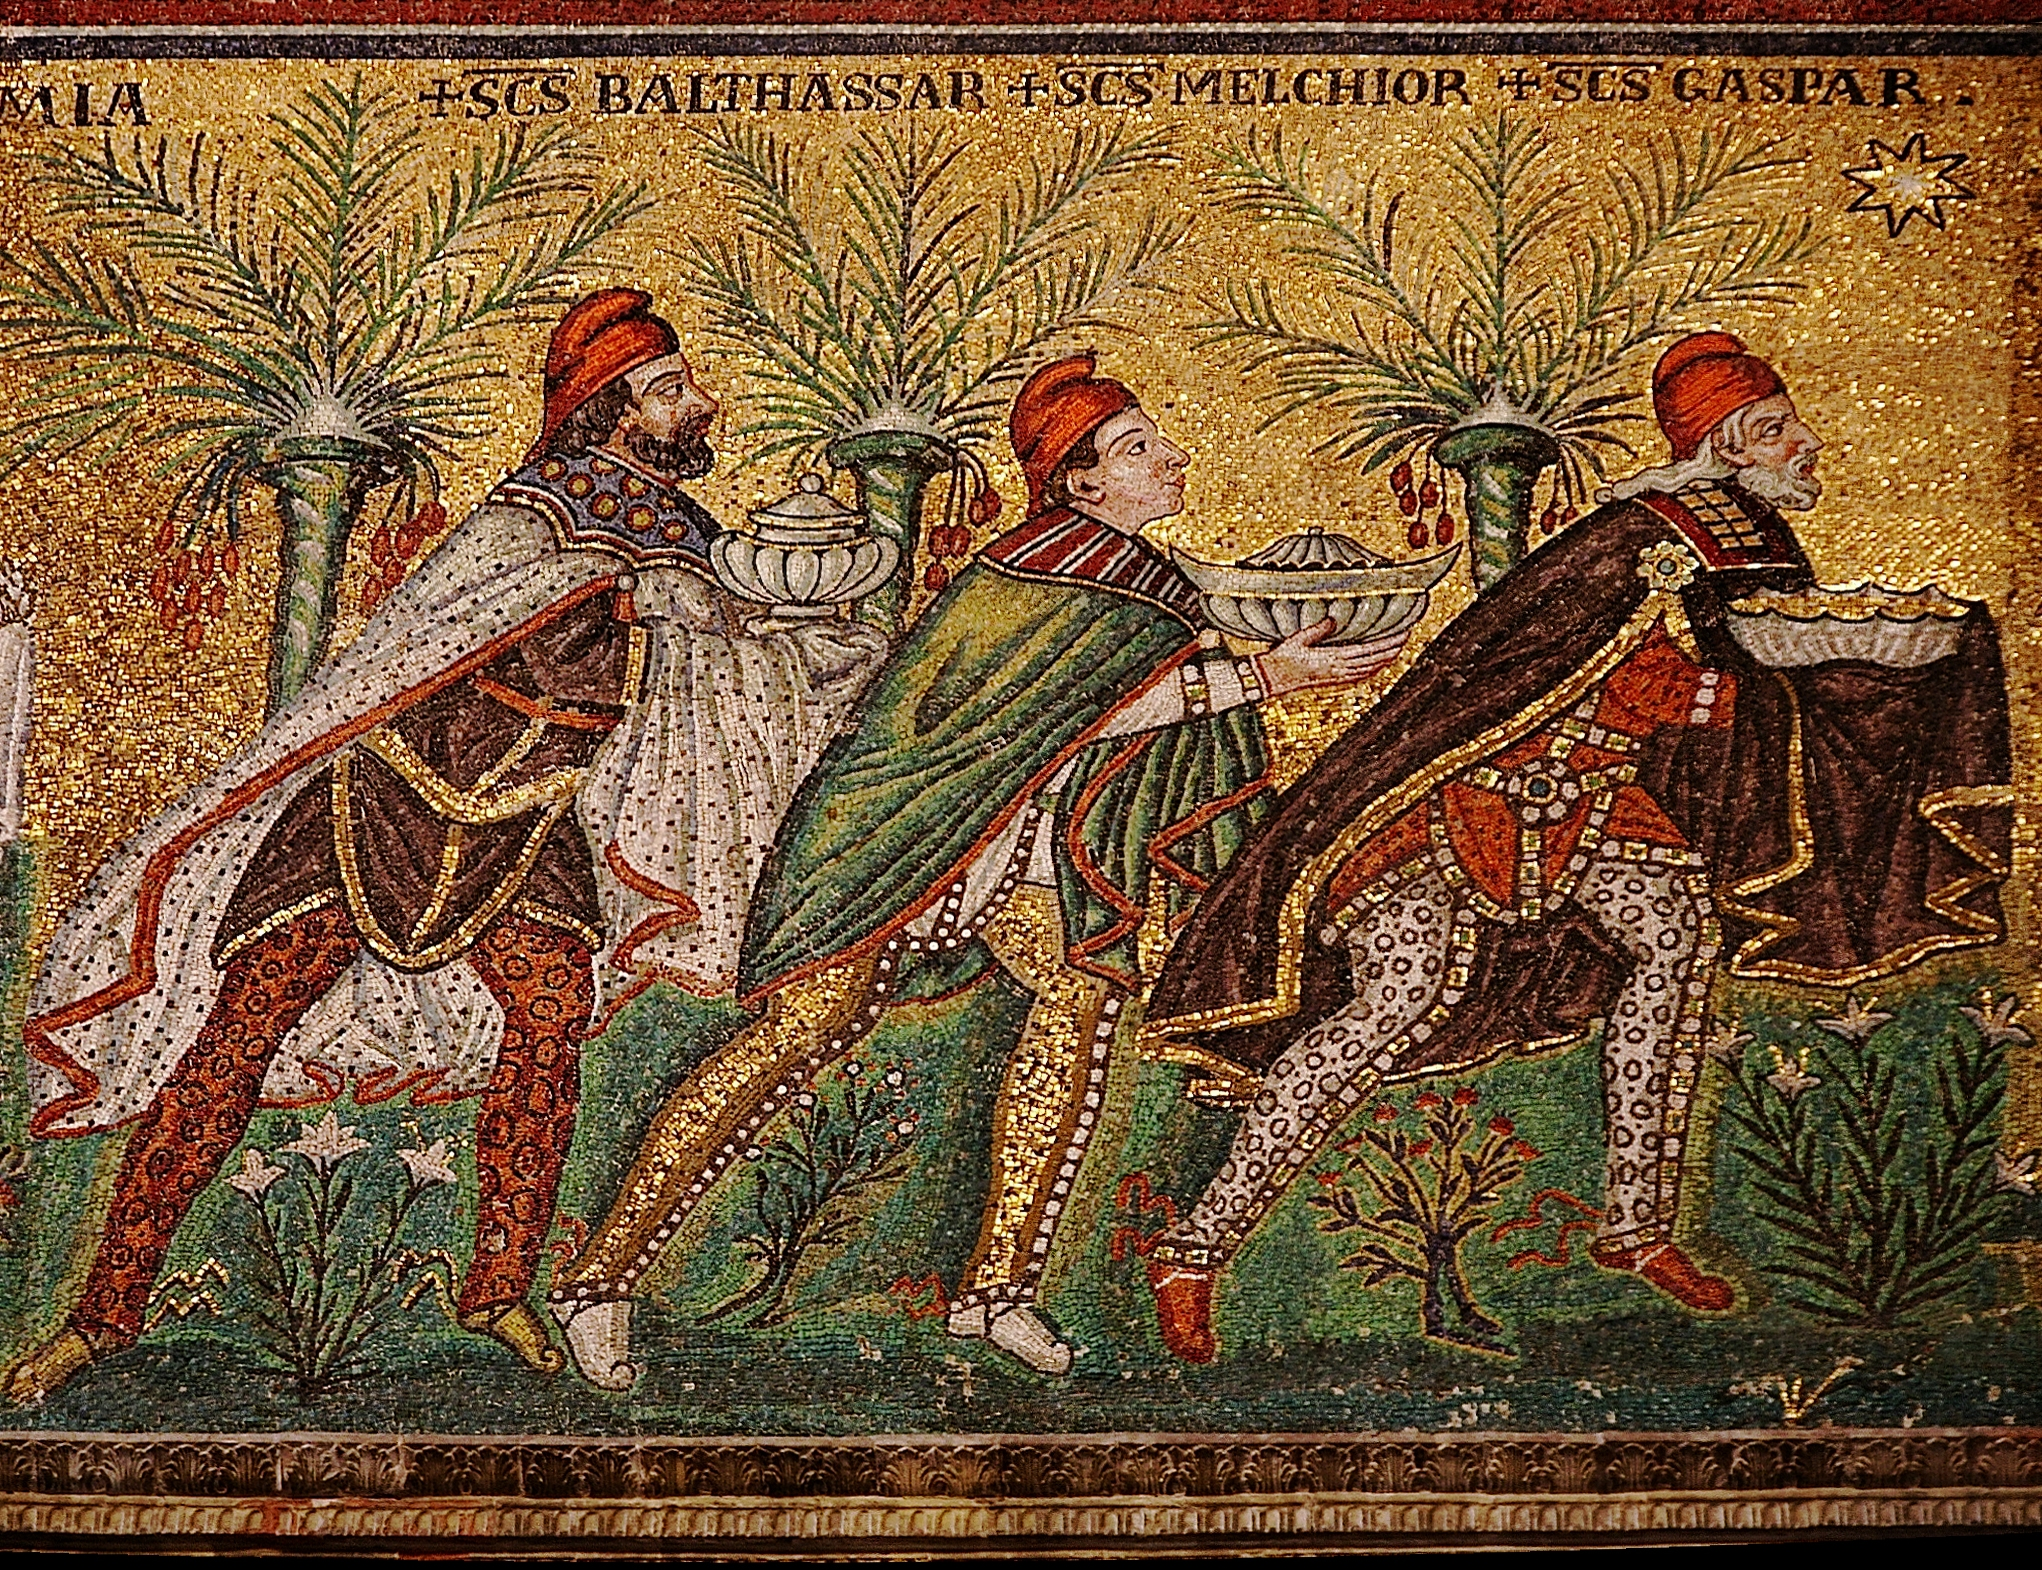
\includegraphics[width=10cm]{imagines/ravenna.jpg}
\end{center}

\vfill

\begin{center}
Ad usum et secundum consuetudines chori \guillemotright{}Conventus Choralis\guillemotleft.

Editio Sancti Wolfgangi \annusEditionis
\end{center}

\pagebreak

\renewcommand{\headrulewidth}{0pt} % no horiz. rule at the header
\fancyhf{}
\pagestyle{fancy}

\pars{Léctio sancti Evangélii secúndum Matthǽum.} \scriptura{Matth. 2, 1-12}

\textusEtTranslatio{
  Cum natus esset Jesus in Béthlehem Juda in diébus Heródis regis,
  ecce Magi ab Oriénte venérunt Jerosólymam, dicéntes:
  Ubi est qui natus est Rex Judæórum?
  Vídimus enim stellam ejus in Oriénte,
  et vénimus adoráre eum.
  Audiens autem Heródes rex, turbátus est,
  et omnis Jerosólyma cum illo.
  Et cóngregans omnes príncipes sacerdótum, et scribas pópuli,
  sci\-sci\-ta\-bá\-tur ab eis, ubi Christus nascerétur.
  At illi dixérunt ei: In Béthlehem Judæ: sic enim scriptum est per Prophétam:
  Et tu Béthlehem terra Juda, nequáquam mínima es in princípibus Juda:
  ex te enim éxiet dux, qui regat pópulum meum Israël.
  Tunc Heródes, clam vocátis Magis, diligénter dídicit ab eis tempus stellæ, quæ appáruit eis:
  Et mittens illos in Béthlehem, dixit: Ite, et interrogate diligénter de púero:
  et cum invenéritis, renuntiáte mihi, ut et ego véniens adórem eum.
  Qui cum audíssent regem, abiérunt, et ecce stella, quam víderant in Oriénte,
  antecedébat eos, usque dum véniens staret supra, ubi erat puer.
  Vidéntes autem stellam gavísi sunt gáudio magno valde.
  Et intrántes domum, invenérunt púerum cum María matre ejus, et procidéntes adoravérunt eum:
  et apértis thesáuris suis obtulérunt ei múnera, aurum, thus et myrrham.
  Et respónso accépto in somnis, ne redírent ad Heródem,
  per áliam viam revérsi sunt in regiónem suam.
}{\trMatEvangelium}{10cm}

\vfill
\pagebreak

\pars{Oratio ante divinum Officium.}

\lettrine{{\color{red}A}}{peri,} Dómine, os meum ad benedicéndum nomen sanctum tuum:
munda quoque cor meum ab ómnibus vanis, pervérsis, et aliénis
cogitatiónibus:
intelléctum illúmina, afféctum inflámma,
ut digne, atténte ac devóte hoc Offícium recitáre váleam,
et exaudíri mérear ante conspéctum Divínæ Majestátis tuæ.
Per Christum, Dominum nostrum.
\Rbardot{} Amen.

Dómine, in unióne illíus divínæ intentiónis,
qua ipse in terris laudes Deo persolvísti,
has tibi Horas \rubricatum{(vel \textnormal{hanc tibi Horam})} persólvo.

\trOratioAnteOfficium

\vfill

\pars{Oratio post divinum Officium.}

\rubrica{
  Orationem sequentem devote post Officium recitantibus
  Leo Papa X. defectus, et culpas in eo persolvendo ex humana
  fragilitate contractas, indulsit, et dicitur flexis genibus.
}

\lettrine{{\color{red}S}}{acrosánctæ} et indivíduæ Trinitáti,
crucifíxi Dómini nostri Jesu Christi humanitáti,
beatíssimæ et gloriosíssimæ sempérque Vírginis Maríæ
fecúndæ integritáti, 
et ómnium Sanctórum universitáti
sit sempitérna laus, honor, virtus et glória
ab omni creatúra,
nobísque remíssio ómnium peccatórum,
per infiníta sǽcula sæculórum.
\Rbardot{} Amen.

\noindent \Vbardot{} Beáta víscera Maríæ Virginis, quæ portavérunt
ætérni Patris Fílium.\\
\Rbardot{} Et beáta úbera, quæ lactavérunt Christum Dominum.

\rubrica{Et dicitur secreto \textnormal{Pater noster.} et \textnormal{Ave María.}}

\trOratioPostOfficium

\vfill

\hora{In Vesperis.} %%%%%%%%%%%%%%%%%%%%%%%%%%%%%%%%%%%%%%%%%%%%%%%%%%%%%
\sideThumbs{Vesperis}

\cantusSineNeumas

\label{deusinadiutorium}

\includescore{temporalia/deusinadiutorium-solemnis.tex}

\vfill
\pagebreak

\cantusCumNeumis

\pars{psalmus 1.} \scriptura{\textbf{H76}}

\antiphona{II D}{temporalia/ant1.tex}

\trAntI

\cantusSineNeumas

\scriptura{Psalmus 109.}

\includescore{temporalia/ps109-initium-ii-D-auto.tex}

\psalmusEtTranslatioT{temporalia/ps109-comb.tex}{10cm}

\vfill
\pagebreak

\pars{psalmus 2.} \scriptura{\textbf{H72}}

\antiphona{I g2}{temporalia/ant2.tex}

\trAntII

\scriptura{Psalmus 110.}

\includescore{temporalia/ps110-initium-i-g2-auto.tex}

\psalmusEtTranslatioT{temporalia/ps110-comb.tex}{10cm}

\vfill
\pagebreak

\pars{psalmus 3.} \scriptura{\textbf{H76}}

\antiphona{I g3}{temporalia/ant3.tex}

\trAntIII

\scriptura{Psalmus 111.}

\includescore{temporalia/ps111-initium-i-g3-auto.tex}

\psalmusEtTranslatioT{temporalia/ps111-comb.tex}{10cm}

\vfill
\pagebreak

\pars{psalmus 4.} \scriptura{\textbf{H76}}

\antiphona{IV E}{temporalia/ant4.tex}

\trAntIV

\scriptura{Psalmus 112.}

\includescore{temporalia/ps112-initium-iv-E-auto.tex}

\psalmusEtTranslatioT{temporalia/ps112-comb.tex}{10cm}

\vfill
\pagebreak

\rubrica{In I. Vesperis:}

\pars{psalmus 5.} \scriptura{\textbf{H77}}

\antiphona{VII c2}{temporalia/ant5.tex}

\trAntV

\scriptura{Psalmus 116.}

\includescore{temporalia/ps116-initium-vii-c2-auto.tex}

\psalmusEtTranslatioT{temporalia/ps116-comb.tex}{10cm}

\vfill
\pagebreak

\rubrica{In II. Vesperis:}

\pars{psalmus 5.} \scriptura{\textbf{H77}}

\antiphona{VII c2}{temporalia/ant5.tex}

\trAntV

\scriptura{Psalmus 113.}

\includescore{temporalia/ps113-initium-vii-c2-auto.tex}

\psalmusEtTranslatioT{temporalia/ps113-comb.tex}{10cm}

\vfill
\pagebreak

\raggedcolumns

% Capitulum. %%%
\cantusSineNeumas

\label{capitulum}
\pars{Capitulum.} \scriptura{Isaiæ 60, 1}

\includescore{temporalia/capitulum-Surge.tex}

% preklad Jeruz. bible
\trCapituli

\vspace{1cm}
\pars{Responsorium breve.}

\superInitialam{VI}
\includescore{temporalia/resp1v.tex}

\trRespVesp

\vfill
\pagebreak

% Hymnus. %%%
\pars{Hymnus.}

\superInitialam{III}
%\includescore{temporalia/hym-HostisHerodes.tex}
%\begin{translatioMulticol}{5}
Lorem ipsum dolor sit amet,\\
consectetur adipiscing elit,\\
sed do eiusmod tempor incididunt\\
ut labore et dolore magna aliqua.\columnbreak

Ut enim ad minim veniam,\\
quis nostrud exercitation\\
ullamco laboris nisi ut\\
aliquip ex ea commodo consequat.\columnbreak

Duis aute irure dolor\\
in reprehenderit in voluptate\\
velit esse cillum dolore eu\\
fugiat nulla pariatur.\columnbreak

Excepteur sint occaecat\\
cupidatat non proident,\\
sunt in culpa qui officia\\
deserunt mollit anim id est laborum.\columnbreak

Sláva tobě, Pane,\\
jenž ses dnes zjevil,\\
s Otcem i Svatým Duchem\\
na věčné věky.
Amen.
\end{translatioMulticol}

\includescore{temporalia/hym-CrudelisHerodes.tex}
\begin{translatioMulticol}{3}
{\color{red}\textit{1.}} Herode krutý, Božího\\
nač se obáváš příchodu?\\
Kdo věčné dává království,\\
neschvátí tvé zdejší štěstí.\\
\\
{\color{red}\textit{2.}} Šli mágové, kde viděli\\
před sebou hvězdu předcházet;\\
za světlem světlo hledají,\\
Boha dary uctívají.\columnbreak

{\color{red}\textit{3.}} Do víru čisté koupele,\\
nebeský vstoupil Beránek:\\
Z hříchů, jež ho netížily,\\
nás obmyl ze své síly.\\
\\
{\color{red}\textit{4.}} Neznámý, nový moci div:\\
ve štoudvích voda zrumění,\\
a když ji nalít poručí\\
tvářnost ve víno promění.\columnbreak

{\color{red}\textit{5.}} Tobě buď sláva, Ježíši,\\
národům že ses projevil,\\
Otci i Duchu života\\
po věkoucí věky světa.\\
Amen.
\end{translatioMulticol}


\vfill

\pagebreak

\pars{Versus.}

% Versus. %%%
\includescore{temporalia/versus-reges.tex}

\noindent \trVersus

\vfill

\cantusCumNeumis

\pars{Canticum B. Mariæ V.}\rubrica{ - in I. vesperis:} \scriptura{\textbf{H76}}

\antiphona{VIII G2}{temporalia/ant-magn-vesp1.tex}

\trAntMagnificatI

\vfill

\pagebreak

\scriptura{Lucæ 1, 46-55}

\cantusSineNeumas
\includescore{temporalia/magnificat-initium-viii-G2.tex}

\psalmusEtTranslatioT{temporalia/magnificat-comb.tex}{10cm}

\pagebreak

\pars{Canticum B. Mariæ V.}\rubrica{ - in II. vesperis:} \scriptura{\textbf{H77}}
\label{magnificatIIvesp}

\cantusCumNeumis

\antiphona{I D*}{temporalia/ant-magn-vesp2.tex}

\trAntMagnificatII

\vfill

\pagebreak

\scriptura{Lucæ 1, 46-55}

\cantusSineNeumas
\includescore{temporalia/magnificat-initium-i-D_.tex}

% maly svindl, ale prizvukova struktura VIIIsoll-G2 a Isoll-D* je stejna
\psalmusEtTranslatioT{temporalia/magnificat-comb.tex}{10cm}

\vfill

\pagebreak

\label{oratio}
\anteOrationem

\pagebreak

% Oratio. %%%
\pars{Oratio.}

\includescore{temporalia/oratio.tex}
\trOrationis

\vspace{1cm}
\rubrica{Hebdomadarius dicit iterum Dominus vobiscum. Postea cantatur a cantore:}
\vspace{2mm}

\rubrica{In I. Vesperis:}

\includescore{temporalia/benedicamus-solemnis-1vesp.tex}

\rubrica{In II. Vesperis:}

\includescore{temporalia/benedicamus-solemnis-2vesp.tex}

\vfill
\pagebreak

\hora{Ad Completorium.} %%%%%%%%%%%%%%%%%%%%%%%%%%%%%%%%%%%%%%%%%%%%%%%%%%%%%%%%%%
\sideThumbs{{\scriptsize{}Completorium}}

\rubrica{Lector petit benedictionem, dicens:}

\includescore{temporalia/jubedomnebenedicere.tex}

\vfill

\pars{Benedictio.}

\includescore{temporalia/benedictio-noctemquietam.tex}

\vfill

\pars{Lectio brevis.} \scriptura{1 Petr. 5, 8-9}

\includescore{temporalia/lectiobrevis-fratressobrii.tex}

\trComplLectioBr

\vfill

\noindent \Vbardot{} Adjutórium nostrum in nómine Dómini. \Rbardot{} Qui fecit cælum, et terram.

\vfill

\noindent Pater noster \rubricatum{quod dicitur totum secreto.}

\vfill
\pagebreak

\pars{Confessio.}

\noindent Confíteor Deo omnipoténti, beátæ Maríæ semper Vírgini, beáto
Michaéli Archángelo, beáto Joánni Baptístæ, sanctis Apóstolis Petro
et Paulo, ómnibus Sanctis, et vobis fratres: quia peccávi nimis cogitatióne,
verbo et ópere: mea culpa, mea culpa, mea máxima culpa.
Ídeo precor beátam Maríam semper Vírginem, beátum Michaélum
Archángelum, beátum Joánnem Baptístam, sanctos Apóstolos Petrum
et Paulum, omnes Sanctos, et vos fratres, oráre pro me ad Dóminum
Deum nostrum.

\vfill

\noindent Misereátur nostri omnípotens Deus, et, dimíssis peccátis nostris, perdúcat
nos ad vitam ætérnam. \Rbardot{} Amen.

\vfill

\noindent Indulgéntiam, absolutiónem et remissiónem peccatórum nostrórum tríbuat nobis
omnípotens et miséricors Dóminus. \Rbardot{} Amen.

\vfill

\rubrica{Et facta absolutione dicitur:}

\includescore{temporalia/convertenosdeus.tex}

\vfill

\includescore{temporalia/deusinadiutorium-communis.tex}

\vfill
\pagebreak

\pars{psalmus 1.}

\antiphona{VIII G}{temporalia/ant-miserere.tex}

\trComplAntI

\scriptura{Psalmus 4.}

\includescore{temporalia/ps4-initium-viii-G-auto.tex}

\psalmusEtTranslatioT{temporalia/ps4-comb.tex}{10cm}

\vfill
\pagebreak

\pars{psalmus 2.} \scriptura{Psalmus 90.}

%\includescore{temporalia/ps90-initium-viii-G-auto.tex}

\psalmusEtTranslatioT{temporalia/ps90-comb.tex}{10cm}

\pagebreak

\pars{psalmus 3.} \scriptura{Psalmus 133.}

%\includescore{temporalia/ps133-initium-viii-G-auto.tex}

\psalmusEtTranslatioT{temporalia/ps133-comb.tex}{10cm}

\vfill

\antiphona{VIII G}{temporalia/ant-miserere.tex}

\vfill

\pars{Hymnus}

\antiphona{VIII}{temporalia/hym-TeLucis.tex}
\begin{translatioMulticol}{3}
Než světlo zhasne prosíme\\
Tebe tvůrce všech pokorně,\\
abys nám ve své milosti\\
byl ochranou a~pomocí.\columnbreak

Ať vzdáleny jsou od nás sny\\
a~těžké noční přízraky.\\
Zdrť našeho nepřítele,\\
těla poskvrn ať ujdeme.\columnbreak

Tobě buď sláva, Ježíši,\\
národům že ses projevil,\\
Otci i~Duchu života\\
po věkoucí věky světa.\\
Amen.
\end{translatioMulticol}


\pagebreak

\pars{Capitulum.} \scriptura{Jer. 14, 9}

\includescore{temporalia/capitulum-tuautem.tex}

% preklad Jeruz. bible
\trComplCapituli

\vfill

\pars{Responsorium breve.} \scriptura{Psalmus 30, 6}

\superInitialam{VI}
\includescore{temporalia/resp-inmanus.tex}

\trRespCompl
\vfill

\pars{Versus.} \scriptura{Psalmus 16, 8}

\includescore{temporalia/versus-custodi.tex}

\noindent \trComplVersus

\vfill
\pagebreak

\cantusCumNeumis

\pars{Canticum Simeonis.}

\antiphona{III a}{temporalia/ant-salvanos-antiquo.tex}

\trAntSalvaNos

\scriptura{Lucæ 2, 29-32}

\includescore{temporalia/nuncdimittis-initium-iii-a-auto.tex}

\psalmusEtTranslatioT{temporalia/nuncdimittis-comb.tex}{10cm}

\vfill
\pagebreak

\pars{Oratio.}

\cantusSineNeumas

\includescore{temporalia/oratio-visita.tex}

\trComplOrationis

\vfill

\includescore{temporalia/domineexaudi.tex}

\vfill

\includescore{temporalia/benedicamus-minor.tex}

\vfill

\pars{Benedictio.}

\noindent Benedícat et custódiat nos omnípotens et miséricors Dóminus, \gredagger{}
Pater, et Fílius, et Spíritus Sanctus. \Rbardot{} Amen.

\vfill
\pagebreak

\pars{Antiphona finalis B. M. V.}

\antiphona{V}{temporalia/an_alma_redemptoris_mater.tex}

\trAlmaRedemptoris

\vfill
\pagebreak

\hora{Ad Matutinum.} %%%%%%%%%%%%%%%%%%%%%%%%%%%%%%%%%%%%%%%%%%%%%%%%%%%%%%%%%%
\sideThumbs{Matutinum}

\subhora{In I. Nocturno}

\pars{psalmus 1.} \scriptura{Psalmus 28, 1.2; \textbf{H72}}

\antiphona{VII a}{temporalia/matant1.tex}

\trMatAntI

\scriptura{Psalmus 28.}

\includescore{temporalia/ps28-initium-vii-a-auto.tex}

\psalmusEtTranslatioT{temporalia/ps28-comb.tex}{10cm}

\vfill
\pagebreak

\pars{psalmus 2.} \scriptura{Psalmus 45, 5; \textbf{H72}}

\antiphona{VI F}{temporalia/matant2.tex}

\trMatAntII

\scriptura{Psalmus 45.}

\includescore{temporalia/ps45-initium-vi-F-auto.tex}

\psalmusEtTranslatioT{temporalia/ps45-comb.tex}{10cm}

\vfill
\pagebreak

\pars{psalmus 3.} \scriptura{Psalmus 46, 7.8; \textbf{H72}}

\antiphona{I f}{temporalia/matant3.tex}

\trMatAntIII

\scriptura{Psalmus 46.}

\includescore{temporalia/ps46-initium-i-f-auto.tex}

\psalmusEtTranslatioT{temporalia/ps46-comb.tex}{10cm}

\vfill
\pagebreak

\pars{Versus.} \scriptura{Psalmus 65, 4}

\includescore{temporalia/versus-omnis.tex}

\noindent \trMatVersusI

\vfill

\includescore{temporalia/oratiodominica-mat.tex}

\vfill

\pars{Absolutio.}

\includescore{temporalia/absolutio-exaudi.tex}

\trMatAbsolutioI

\vfill
\pagebreak

\includescore{temporalia/benedictio-solemn-benedictione.tex}

\trMatBenedictioI

\vfill

\includescore{temporalia/tonus-lectionis-solemnis.tex}

\vfill

% De Isaia Prophéta.
\pars{Lectio I} \scriptura{Isaiæ 55, 1-4}

\noindent De Isaia \textit{Pro}phéta.

\textusEtTranslatio{
  Omnes siti\textbf{én}tes,~\gredagger{}
  vení\textit{te} ad aquas,~\grestar{}
  et qui non habétis ar\textbf{gén}tum,~\gredagger{}
  properáte, émite, \textit{et} comédite:~\grestar{}
  veníte, émite absque argénto et absque ulla commutatióne vi\textit{num} et lac.
  Quare appénditis argéntum non in pánibus,
  \textit{et} labórem vestrum non in satu\textit{ri}táte?
  Audíte, audi\textbf{én}tes me,~\gredagger{}
  et comé\textit{di}te bonum,~\grestar{}
  et delectábitur in crassitúdine áni\textit{ma} vestra.
  Inclináte aurem vestram, et veníte \textbf{ad} me;~\gredagger{}
  audíte, et vivet á\textit{ni}ma vestra,~\grestar{}
  et fériam vobíscum pactum sempitérnum, misericórdias David \textit{fi}déles.
  Ecce testem pópulis \textit{de}di eum,~\grestar{}
  ducem ac præceptó\textit{rem} géntibus.
}{\trMatLecI}{10cm}

\tuAutem

\vfill
\pagebreak

\pars{Responsorium 1.} \scriptura{\Rbar{} Matth. 3, 16-17 \Vbar{} Lucæ 3, 22; \textbf{H72}}

\responsorium{III}{temporalia/matresp1.tex}{\trMatRespI}

\vfill
\pagebreak

\includescore{temporalia/benedictio-solemn-unigenitus.tex}

\trMatBenedictioII

\vfill

\pars{Lectio II} \scriptura{Isaiæ 60, 1-6}

\textusEtTranslatio{
  Surge, illumináre, Je\textbf{rú}salem,~\gredagger{}
  quia venit \textit{lu}men tuum,~\grestar{}
  et glória Dómini super \textbf{te} orta est.
  Quia ecce ténebræ opérient terram, et calígo \textbf{pó}pulos;~\gredagger{}
  super te autem ori\textit{é}tur Dóminus,~\grestar{}
  et glória ejus in te \textit{vi}débitur.
  Et ambulábunt gentes in lú\textit{mi}ne tuo,~\grestar{}
  et reges in splendóre or\textit{tus} tui.
  Leva in circúitu óculos tuos, et \textbf{vi}de:~\gredagger{}
  omnes isti congregáti sunt, ve\textit{né}runt \hbox{tibi;~\grestar{}}
  fílii tui de longe vénient et fíliæ tuæ de láte\textit{re} surgent.
  Tunc vidébis, et áfflues; mirábitur et dilatábitur cor \textbf{tu}um:~\gredagger{}
  quando convérsa fúerit ad te multi\textit{tú}do maris;~\grestar{}
  fortitúdo géntium véne\textit{rit} tibi.
  Inundátio camelórum opériet te, dromedárii Mádian et \textbf{E}pha;~\gredagger{}
  omnes de Saba vénient, aurum et thus \textit{de}feréntes,~\grestar{}
  et laudem Dómino annun\textit{ti}ántes.
}{\trMatLecII}{10cm}

\tuAutem

\vfill
\pagebreak

\pars{Responsorium 2.} \scriptura{\Rbar{} Matth. 3, 16-17 \Vbar{} ibidem; \textbf{H75}}

\responsorium{II}{temporalia/matresp2.tex}{\trMatRespII}

\vfill
\pagebreak

\includescore{temporalia/benedictio-solemn-spiritus.tex}

\trMatBenedictioIII

\vfill

\pars{Lectio III} \scriptura{Isaiæ 61, 10-11; 62, 1}

\textusEtTranslatio{
  Gaudens gaudébo in \textbf{Dó}mino,~\gredagger{}
  et exsultábit ánima mea in \textit{De}o meo,~\grestar{}
  quia índuit me vestiméntis sa\textbf{lú}tis,~\gredagger{}
  et induménto justítiæ circúmdedit me, quasi sponsum decorá\textit{tum} coróna,~\grestar{}
  et quasi sponsam ornátam moníli\textit{bus} suis.
  Sicut enim terra profert germen \textbf{su}um,~\gredagger{}
  et sicut hortus semen \textit{su}um gérminat,~\grestar{}
  sic Dóminus Deus germinábit justítiam et laudem coram univér\textit{sis} géntibus.
  Propter Sion non tacébo, et propter Jerúsalem non qui\textbf{és}cam,~\gredagger{}
  donec egrediátur ut splendor \textit{jus}tus ejus,~\grestar{}
  et salvátor ejus ut lampas ac\textit{cen}dátur.
}{\trMatLecIII}{10cm}

\tuAutem

\vfill
\pagebreak

\pars{Responsorium 3.} \scriptura{\Rbar{} Psalmus 71, 10 \Vbar{} Isaiæ 60, 6; \textbf{Sar. 85}}

\responsorium{II}{temporalia/matresp3.tex}{\trMatRespIII}

\vfill
\pagebreak

\subhora{In II. Nocturno}

\pars{psalmus 4.} \scriptura{Psalmus 65, 4; \textbf{H73}}

\antiphona{IV E}{temporalia/matant4.tex}

\trMatAntIV

\scriptura{Psalmus 65.}

\includescore{temporalia/ps65-initium-iv-E-auto.tex}

\psalmusEtTranslatioT{temporalia/ps65-comb.tex}{10cm}

\vfill
\pagebreak

\pars{psalmus 5.} \scriptura{Psalmus 71, 10; \textbf{H73}}

\antiphona{I a2}{temporalia/matant5.tex}

\trMatAntV

\scriptura{Psalmus 71.}

\includescore{temporalia/ps71-initium-i-a2-auto.tex}

\psalmusEtTranslatioT{temporalia/ps71-comb.tex}{10cm}

\vfill
\pagebreak

\pars{psalmus 6.} \scriptura{Psalmus 85, 7.8; \textbf{H73}}

\antiphona{IV E}{temporalia/matant6.tex}

\trMatAntVI

\scriptura{Psalmus 85.}

\includescore{temporalia/ps85-initium-iv-E-auto.tex}

\psalmusEtTranslatioT{temporalia/ps85-comb.tex}{10cm}

\vfill
\pagebreak

\pars{Versus.}

\includescore{temporalia/versus-reges.tex}

\noindent \trVersus

\vfill

\includescore{temporalia/oratiodominica-mat.tex}

\vfill

\pars{Absolutio.}

\includescore{temporalia/absolutio-ipsius.tex}

\trMatAbsolutioII

\vfill
\pagebreak

\includescore{temporalia/benedictio-solemn-deus.tex}

\trMatBenedictioIV

\vfill

% Sermo sancti Leónis Papæ.
\pars{Lectio IV} \scriptura{Sermo 2. de Epiphania.}

\noindent Sermo sancti Leó\textit{nis} Papæ.

\textusEtTranslatio{
  Gaudéte in Dómino, dilec\textbf{tís}simi,~\gredagger{}
  íterum di\textit{co,} gaudéte:~\grestar{}
  quóniam brevi intervállo témporis, post solemnitátem Nativitátis \textbf{Chris}ti,~\gredagger{}
  festívitas declaratiónis ejus illúxit: et quem in illo die \textit{Vir}go péperit,~\grestar{}
  in hoc mundus \textit{ag}nóvit.
  Verbum enim caro factum, sic susceptiónis nostræ temperávit e\textbf{xór}dia,~\gredagger{}
  ut natus Jesus et credéntibus \textit{ma}niféstus,~\grestar{}
  et persequéntibus esset \textit{oc}cúltus.
  Jam tunc ergo cæli enarravérunt glóriam \textbf{De}i,~\gredagger{}
  et in omnem terram sonus veritá\textit{tis} exívit,~\grestar{}
  quando et pastóribus exércitus Angelórum Salvatóris éditi annuntiátor ap\textbf{pá}ruit,~\gredagger{}
  et Magos ad eum adorándum prǽvia stel\textit{la} perdúxit:~\grestar{}
  ut a solis ortu usque ad occásum veri Regis generátio corus\textbf{cá}ret,~\gredagger{}
  cum rerum fidem et regna Oriéntis per \textit{Ma}gos díscerent,~\grestar{}
  et Románum impérium \textit{non} láteret.
}{\trMatLecIV}{10cm}

\tuAutem

\vfill
\pagebreak

\pars{Responsorium 4.} \scriptura{\Rbar{} Isaiæ 60, 1 \Vbar{} ibid. 60, 3; \textbf{H74}}

\responsorium{V}{temporalia/matresp4.tex}{\trMatRespIV}

\vfill
\pagebreak

\includescore{temporalia/benedictio-solemn-christus.tex}

\trMatBenedictioV

\vfill

\pars{Lectio V} \scriptura{Sermo 2. de Epiphania.}

\textusEtTranslatio{
  Nam et sævítia Heródis volens primórdia suspécti sibi Regis exs\textbf{tín}guere,~\gredagger{}
  huic dispensatíoni nésciens serviébat: ut dum atróci intén\textit{tus} facínori,~\grestar{}
  ignótum sibi púerum indiscréta infántium cæde per\textbf{sé}quitur,~\gredagger{}
  annuntiátum cǽlitus dominatóris ortum insígnior ubíque fama \textit{lo}querétur:~\grestar{}
  quam promptiórem ad nar\textbf{rán}dum,~\gredagger{}
  diligentiorémque faciébat et supérnæ significati\textit{ó}nis nóvitas,~\grestar{}
  et cruentíssimi persecutóris \textit{im}píetas.
  Tunc autem étiam Ægýpto Salvátor il\textbf{lá}tus est,~\gredagger{}
  ut gens antíquis erró\textit{ri}bus dédita,~\grestar{}
  jam ad vicínam salútem per occúltam grátiam signa\textbf{ré}tur:~\gredagger{}
  et quæ nondum ejécerat ab ánimo super\textit{sti}tiónem,~\grestar{}
  jam hospítio recíperet ve\textit{ri}tátem.
}{\trMatLecV}{10cm}

\tuAutem

\vfill
\pagebreak

\pars{Responsorium 5.} \scriptura{\Rbar{} Isaiæ 60, 6 \Vbar{} Psalmus 71, 10; \textbf{H73}}

\responsorium{VII}{temporalia/matresp5.tex}{\trMatRespV}

\vfill
\pagebreak

\includescore{temporalia/benedictio-solemn-ignem.tex}

\trMatBenedictioVI

\vfill

\pars{Lectio VI} \scriptura{Sermo 2. de Epiphania.}

\textusEtTranslatio{
  Agnoscámus ergo, dilec\textbf{tís}simi,~\gredagger{}
  in Magis adoratóribus Christi, vocatiónis nostræ fideí\textit{que} primítias:~\grestar{}
  et exsultántibus ánimis beátæ spei inítia ce\textit{leb}rémus.
  Exínde enim in ætérnam hereditátem cœpimus intro\textbf{í}re:~\gredagger{}
  exínde nobis Christum loquéntia Scripturárum arcána patué\textit{runt,} et \hbox{véritas,~\grestar{}}
  quam Judæórum obcæcátio non récipit, ómnibus natiónibus lumen suum \textit{in}véxit.
  Honorétur ítaque a nobis sacratíssimus dies, in quo salútis nostræ Auctor ap\textbf{pá}ruit:~\gredagger{}
  et quem Magi infántem veneráti sunt \textit{in} cunábulis,~\grestar{}
  nos omnipoténtem adorémus in cælis.
  Ac sicut illi de thesáuris suis mýsticas Dómino múnerum spécies obtu\textbf{lé}runt,~\gredagger{}
  ita et nos de cór\textit{di}bus nostris,~\grestar{}
  quæ Deo sunt digna, \textit{pro}mámus.
}{\trMatLecVI}{10cm}

\tuAutem

\vfill
\pagebreak

\pars{Responsorium 6.} \scriptura{\Rbar{} Matth. 2, 1-2 \Vbar{} ibidem 2, 2; \textbf{H74}}

\responsorium{VIII}{temporalia/matresp6.tex}{\trMatRespVI}

\vfill
\pagebreak

\subhora{In III. Nocturno}

\pars{psalmus 7.} \scriptura{Psalmus 94, 6.7; \textbf{H74}}

\antiphona{VIII G}{temporalia/matant7.tex}

\trMatAntVII \scriptura{Psalmus 94.}

\includescore{temporalia/ps94-initium-viii-G.tex}

\psalmusEtTranslatioT{temporalia/ps94-comb.tex}{10.5cm}

\vfill
\pagebreak

\pars{psalmus 8.} \scriptura{Psalmus 95, 9; \textbf{H74}}

\antiphona{VI F}{temporalia/matant8.tex}

\trMatAntVIII

\scriptura{Psalmus 95.}

\includescore{temporalia/ps95-initium-vi-F-auto.tex}

\psalmusEtTranslatioT{temporalia/ps95-comb.tex}{10cm}

\vfill
\pagebreak

\pars{psalmus 9.} \scriptura{Psalmus 96, 7; \textbf{H74}}

\antiphona{VI F}{temporalia/matant9.tex}

\trMatAntIX

\scriptura{Psalmus 96.}

\includescore{temporalia/ps96-initium-vi-F-auto.tex}

\psalmusEtTranslatioT{temporalia/ps96-comb.tex}{10cm}

\vfill
\pagebreak

\pars{Versus.} \scriptura{Psalmus 95, 9}

\includescore{temporalia/versus-adorate-mat.tex}

\noindent \trMatVersusIII

\vfill

\includescore{temporalia/oratiodominica-mat.tex}

\vfill

\pars{Absolutio.}

\includescore{temporalia/absolutio-avinculis.tex}

\trMatAbsolutioIII

\vfill
\pagebreak

\includescore{temporalia/benedictio-solemn-evangelica.tex}

\trMatBenedictioVII

\vfill

% Léctio sancti Evangélii secúndum Matthǽum.
\pars{Lectio VII} \scriptura{Matth. 2, 1-12}

\noindent Léctio sancti Evangélii secúndum \textit{Mat}thǽum.

\textusEtTranslatio{
  Cum natus esset Jesus in Béthlehem Juda in diébus Heródis \textbf{re}gis,~\gredagger{}
  ecce Magi ab Oriénte venérunt \textit{Je}rosólymam,~\grestar{}
  dicéntes: \textit{U}bi est qui natus est Rex Ju\textit{dæ}órum?
  \textit{Et} réliqua.
}{\trMatLecVIIa}{10cm}

% Homilía sancti Gregórii Papæ.
\scriptura{Homilia 10. in Evang.}

\noindent Homilía sancti Gregóri\textit{i} Papæ.

\textusEtTranslatio{
  Sicut in lectióne evan\textbf{gé}lica,~\gredagger{}
  fratres caríssi\textit{mi,} audístis,~\grestar{}
  cæli Rege nato, rex terræ tur\textbf{bá}tus est:~\gredagger{}
  quia nimírum terréna altitú\textit{do} confún\-\hbox{ditur,~\grestar{}}
  cum celsitúdo cæléstis a\textit{pe}rítur.
  Sed quæréndum nobis est, quidnam sit, quod, Redemptóre \textbf{na}to,~\gredagger{}
  pastóribus in Judǽa Ange\textit{lus} appáruit,~\grestar{}
  atque ad adorándum hunc ab Oriénte Magos non Angelus, \textit{sed} stella \textit{per}dúxit?
  Quia vidélicet Judǽis, tamquam ratióne uténtibus, rationále \textbf{á}nimal,~\gredagger{}
  id est, Angelus prædi\textit{cá}re débuit:~\grestar{}
  Gentíles vero, quia uti ratióne nesci\textbf{é}bant,~\gredagger{}
  ad cognoscéndum Dóminum \textit{non} per vocem,~\grestar{}
  sed per signa per\textit{du}cúntur.
  Unde étiam per Paulum \textbf{dí}citur:~\gredagger{}
  Prophetíæ fidélibus datæ sunt, non \textit{in}fidéli\-\hbox{bus:~\grestar{}}
  signa autem infidélibus, non \textit{fi}délibus.
  Quia et illis prophetíæ tamquam fidélibus, non infi\textbf{dé}libus:~\gredagger{}
  et istis signa tamquam \textit{in}fidélibus,~\grestar{}
  non fidéli\textit{bus} data sunt.
}{\trMatLecVIIb}{10cm}

\tuAutem

\vfill
\pagebreak

\pars{Responsorium 7.} \scriptura{\Rbar{} Matth. 2, 9-10 \Vbar{} ibid. 2, 11; \textbf{H73}}

\responsorium{VIII}{temporalia/matresp7.tex}{\trMatRespVII}

\vfill
\pagebreak

\includescore{temporalia/benedictio-solemn-divinum.tex}

\trMatBenedictioVIII

\vfill

\pars{Lectio VIII} \scriptura{Homilia 10. in Evang.}

\textusEtTranslatio{
  Et notándum, quod Redemptórem nostrum, cum jam perféctæ esset æ\textbf{tá}tis,~\gredagger{}
  eísdem Gentílibus Apóstoli prǽdicant, \textit{eúm}que párvulum,~\grestar{}
  et necdum per humáni córporis offícium lo\textbf{quén}tem,~\gredagger{}
  stella Génti\textit{bus} denúntiat:~\grestar{}
  quia nimírum ratiónis ordo pos\textbf{cé}bat,~\gredagger{}
  ut et loquéntem jam Dóminum loquéntes nobis prædicatóres \textit{in}notéscerent,~\grestar{}
  et necdum loquéntem eleménta muta præ\textit{di}cárent.
  Sed in ómnibus signis, quæ vel nascénte \textbf{Dó}mino,~\gredagger{}
  vel moriénte eo monstráta sunt, conside\textit{rán}dum nobis est,~\grestar{}
  quanta fúerit in quorúmdam Judæórum corde du\textbf{rí}tia,~\gredagger{}
  qui hunc nec per prophe\textit{tí}æ do\-\hbox{num,~\grestar{}}
  nec per mirácula ag\textit{no}vérunt.
}{\trMatLecVIII}{10cm}

\tuAutem

\vfill
\pagebreak

\pars{Responsorium 8.} \scriptura{\Rbar{} Matth. 2, 10-11 \Vbar{} ibid. 2, 9; \textbf{H75}}

\responsorium{IV}{temporalia/matresp8.tex}{\trMatRespVIII}

\vfill
\pagebreak

\includescore{temporalia/benedictio-solemn-perevangelica.tex}

\trMatBenedictioIX

\vfill

\pars{Lectio IX} \scriptura{Homilia 10. in Evang.}

\textusEtTranslatio{
  Omnia quippe eleménta auctórem suum venísse \textit{tes}táta sunt.
  Ut enim de eis quiddam usu humáno \textbf{lo}quar:~\gredagger{}
  Deum hunc cæli esse \textit{cog}no\-\hbox{vérunt,~\grestar{}}
  quia prótinus stellam \textit{mi}sérunt.
  Ma\textit{re} cognóvit,~\grestar{}
  quia sub plantis ejus se calcábi\textit{le} prǽbuit.
  Ter\textit{ra} cognóvit,~\grestar{}
  quia eo moriénte \textit{con}trémuit.
  Sol cognóvit, quia lucis suæ rádios \textit{abs}cóndit.
  Saxa et paríetes \textit{cog}novérunt,~\grestar{}
  quia témpore mortis e\textit{jus} scissa sunt.
  Inférnus ag\textit{nó}vit, quia hos,~\grestar{}
  quos tenébat mórtu\textit{os,} réddidit.
  Et tamen hunc, quem Dóminum ómnia insensibília eleménta sen\textbf{sé}runt,~\gredagger{}
  adhuc infidélium Judæórum corda Deum esse míni\textit{me} cognóscunt,~\grestar{}
  et durióra saxis, scindi ad pœnitén\textit{dum} nolunt.
}{\trMatLecIX}{10cm}

\tuAutem

\vfill
\pagebreak

% Te Deum

\pars{Hymnus Ambrosianus}

\superInitialam{III}
\includescore{temporalia/tedeum-solemnis.tex}

\trTeDeum

\vfill
\pagebreak

% Evangelium

\includescore{temporalia/tonus-evangelii-b.tex}

\vfill

\pars{Léctio sancti Evangélii secúndum Mat\textit{thǽ}um.} \scriptura{Matth. 2, 1-12}

\textusEtTranslatio{
  Cum natus esset Jesus in Béthlehem Juda in diébus \textit{He}ródis regis,~\grestar{}
  ecce Magi ab Oriénte venérunt Jerosólymam, dicéntes:
  \textit{U}bi est qui natus est Rex \textit{Ju}dæórum?
  Vídimus enim stellam e\textit{jus} in Oriénte,~\grestar{}
  et vénimus adoráre \textbf{e}um.
  Audiens autem Heró\textit{des} rex, turbátus est,~\grestar{}
  et omnis Jerosólyma cum \textbf{il}lo.
  Et cóngregans omnes príncipes sacerdótum, \textit{et} scribas pópuli,~\grestar{}
  sci\-sci\-ta\-bá\-tur ab eis, ubi Christus nasce\textbf{ré}tur.
  At illi dixérunt ei: In Béthlehem Judæ: sic enim scriptum \textit{est} per Prophétam:~\grestar{}
  Et tu Béthlehem terra Juda, nequáquam mínima es in \textit{prin}cípibus Juda:~\grestar{}
  ex te enim éxiet dux, qui regat pópulum meum Is\textbf{ra}ël.
  Tunc Heródes, clam vocátis Magis, diligénter dídicit ab eis tempus stellæ, quæ \textit{ap}páruit eis:~\grestar{}
  Et mittens illos in Béthlehem, dixit: Ite, et interrogate di\textit{li}génter de púero:~\grestar{}
  et cum invenéritis, renuntiáte mihi, ut et ego véniens adórem \textbf{e}um.
  Qui cum audíssent regem, abiérunt, et ecce stella, quam víde\textit{rant} in Oriénte,~\grestar{}
  antecedébat eos, usque dum véniens staret supra, ubi erat \textbf{pu}er.
  Vidéntes autem stellam gavísi sunt gáudio magno \textbf{val}de.
  Et intrántes domum, invenérunt púerum cum María matre ejus, et procidéntes ado\textit{ra}vérunt eum:~\grestar{}
  et apértis thesáuris suis obtulérunt ei múnera, aurum, thus et \textbf{myr}rham.
  Et respónso accépto in somnis, ne redírent ad He\textbf{ró}dem,
  \textit{per} áliam viam revérsi sunt in regiónem \textbf{su}am.
}{\trMatEvangelium}{10cm}

\vfill
\superInitialam{I}
\includescore{temporalia/tedecetlaus.tex}

\trTeDecetLaus

\vfill
\pagebreak

\includescore{temporalia/domineexaudi.tex}

\vfill

\pars{Oratio.}

\includescore{temporalia/oratio.tex}
\trOrationis

\vfill

\noindent \Vbardot{} Dómine, exáudi oratiónem meam.
\Rbardot{} Et clamor meus ad te véniat.

\vfill

% Nocturnale Romanum 2002, p. LXXVI Benedicamus Domino seems to match
% the one from Solemn Laudes.
\includescore{temporalia/benedicamus-solemnis-laud.tex}

\vfill

\noindent \Vbardot{} Fidélium ánimæ per misericórdiam Dei requiéscant in pace.
\Rbardot{} Amen.

\vfill
\pagebreak

\hora{Ad Laudes.} %%%%%%%%%%%%%%%%%%%%%%%%%%%%%%%%%%%%%%%%%%%%%%%%%%%%%%%%%%
\sideThumbs{Laudes}

% Psalmi festivi (AM33, pg. 721):
% 92, 99, 62, Dan3, 148+149+150

\vspace{1cm}
\includescore{temporalia/deusinadiutorium-communis.tex}
\vspace{1cm}

\vfill
\pagebreak

\cantusSineNeumas

\pars{psalmus 1.} \scriptura{\textbf{H76}}

\antiphona{II D}{temporalia/ant1.tex}

\trAntI

\scriptura{Psalmus 92.}

\includescore{temporalia/ps92-initium-ii-D-auto.tex}

\psalmusEtTranslatioT{temporalia/ps92-comb.tex}{10cm}

\vfill
\pagebreak

\pars{psalmus 2.} \scriptura{\textbf{H72}}

\antiphona{I g2}{temporalia/ant2.tex}

\trAntII

\scriptura{Psalmus 99.}

\includescore{temporalia/ps99-initium-i-g2-auto.tex}

\psalmusEtTranslatioT{temporalia/ps99-comb.tex}{10cm}

\vfill
\pagebreak

\pars{psalmus 3.} \scriptura{\textbf{H76}}

\antiphona{I g3}{temporalia/ant3.tex}

\trAntIII

\scriptura{Psalmus 62.}

\includescore{temporalia/ps62-initium-i-g3-auto.tex}

\psalmusEtTranslatioT{temporalia/ps62-comb.tex}{10cm}

\vfill
\pagebreak

\pars{psalmus 4.} \scriptura{\textbf{H76}}

\antiphona{IV E}{temporalia/ant4.tex}

\trAntIV

\scriptura{Canticum trium puerorum, Dan. 3, 57-88 et 56.}

\includescore{temporalia/dan3-initium-iv-E-auto.tex}

\psalmusEtTranslatioT{temporalia/dan3-comb.tex}{10cm}

\rubrica{Hic non dicitur Gloria Patri, neque Amen.}
\vspace{1cm}

\hicSuntNeumae
\includescore{temporalia/ant4.tex} % repeat the antiphon - new page

\vfill
\pagebreak

\pars{psalmus 5.} \scriptura{\textbf{H77}}

\antiphona{VII c2}{temporalia/ant5.tex}

\trAntV

%
\scriptura{Psalmus 148.}

\includescore{temporalia/ps148-initium-vii-c2-auto.tex}

\newlength{\psVItransW}
\setlength{\psVItransW}{10.5cm}

\psalmusEtTranslatioT{temporalia/ps148-comb.tex}{10cm}

\rubrica{Hic non dicitur Gloria Patri.}

%
\scriptura{Psalmus 149.}

\includescore{temporalia/ps149-initium-vii-c2-auto.tex}

\psalmusEtTranslatioT{temporalia/ps149-comb.tex}{10cm}

\rubrica{Hic non dicitur Gloria Patri.}

\vfill
\pagebreak

%
\scriptura{Psalmus 150.}

\includescore{temporalia/ps150-initium-vii-c2-auto.tex}

\psalmusEtTranslatioT{temporalia/ps150-comb.tex}{10cm}

\pagebreak

\cantusSineNeumas

\pars{Capitulum.} \scriptura{Isaiæ 60, 1}

\includescore{temporalia/capitulum-Surge.tex}

% preklad Jeruz. bible
\trCapituli

\vspace{1cm}
\pars{Responsorium breve.}

\superInitialam{VI}
\includescore{temporalia/respl.tex}

\trRespLaudes
\vfill
\pagebreak

\pars{Hymnus.}

\includescore{temporalia/hym-OSolaMagnarum.tex}
%BETHLEHEM! of noblest cities
%none can once with thee compare;
%thou alone the Lord from heaven
%didst for us Incarnate bear.
%
%Fairer than the sun at morning
%was the star that told His birth;
%to the lands their God announcing,
%hid beneath a form of earth.
%
%By its lambent beauty guided,
%see the eastern kings appear;
%see them bend, their gifts to offer-
%gifts of incense, gold, and myrrh.
%
%Solem things of mystic meaning!-
%Incense doth the God disclose;
%Gold a royal Child proclaimeth;
%Myrrh a future tomb foreshows.

\begin{translatioMulticol}{5}
Lorem ipsum dolor sit amet,\\
consectetur adipiscing elit,\\
sed do eiusmod tempor incididunt\\
ut labore et dolore magna aliqua.\columnbreak

Ut enim ad minim veniam,\\
quis nostrud exercitation\\
ullamco laboris nisi ut\\
aliquip ex ea commodo consequat.\columnbreak

Duis aute irure dolor\\
in reprehenderit in voluptate\\
velit esse cillum dolore eu\\
fugiat nulla pariatur.\columnbreak

Excepteur sint occaecat\\
cupidatat non proident,\\
sunt in culpa qui officia\\
deserunt mollit anim id est laborum.\columnbreak

Sláva tobě, Pane,\\
jenž ses dnes zjevil,\\
s Otcem i Svatým Duchem\\
na věčné věky.
Amen.
\end{translatioMulticol}


\vfill
\pagebreak

\pars{Versus.}

% Versus. %%%
\includescore{temporalia/versus-adorate.tex}

\noindent \trVersusLaudes

\vfill

\cantusCumNeumis

\pars{Canticum Zachariæ.} \scriptura{\textbf{H76}}

\antiphona{VIII G2}{temporalia/ant-ben-laud.tex}

\trAntBenedictus

\scriptura{Lucæ 1, 68-79}

\includescore{temporalia/benedictus-initium-viiisoll-G2-auto.tex}

\psalmusEtTranslatioT{temporalia/benedictus-comb.tex}{10cm}

\vfill
\pagebreak

\cantusSineNeumas

\anteOrationem

\pagebreak

% Oratio. %%%
\pars{Oratio.}

\includescore{temporalia/oratio.tex}
\trOrationis

\vspace{1cm}
\rubrica{Hebdomadarius dicit iterum Dominus vobiscum. Postea cantatur a cantore:}
\vspace{2mm}

\includescore{temporalia/benedicamus-solemnis-laud.tex}

\vfill
\pagebreak

\hora{Ad Tertiam.} %%%%%%%%%%%%%%%%%%%%%%%%%%%%%%%%%%%%%%%%%%%%%%%%%%%%%%%%%%
\sideThumbs{Tertia}

\vspace{1cm}
\includescore{temporalia/deusinadiutorium-communis.tex}
\vspace{1cm}

\pars{Hymnus}

\antiphona{VIII}{temporalia/hym-NuncSancte.tex}
\begin{translatioMulticol}{3}
Nyní nás Duchu přesvatý\\
s Otcem a Synem pronikni,\\
v okamžik jediný do srdce\\
vstup a zal\ij{} je milostí.\columnbreak

Ať ústa, jazyk i smysly,\\
mysl a síla vyznají,\\
ať ohněm láska zaplane\\
horlivá ke všem bližním.\columnbreak

Tobě buď sláva, náš Pane,\\
národům že ses projevil,\\
Otci i Duchu života\\
po věkoucí věky světa.\\
Amen.
\end{translatioMulticol}


\vfill
\pagebreak

\pars{psalmus.} \scriptura{\textbf{H72}}

\antiphona{I g2}{temporalia/ant2.tex}

\trAntII

\scriptura{Psalmus 118. {\hebfont{ה}},{\hebfont{ו}},{\hebfont{ז}},{\hebfont{ח}},{\hebfont{ט}},{\hebfont{י}}}

\includescore{temporalia/ps118v_x-initium-i-g2-auto.tex}

\psalmusEtTranslatioT{temporalia/ps118v_x-comb.tex}{10cm}

% \antiphona{I g2}{temporalia/ant2.tex}

\vfill
\pagebreak

\raggedcolumns

% Capitulum. %%%
\cantusSineNeumas

\label{capitulum}
\pars{Capitulum.} \scriptura{Isaiæ 60, 1}

\includescore{temporalia/capitulum-Surge.tex}

% preklad Jeruz. bible
\trCapituli

\vfill

\pars{Versus.}

\includescore{temporalia/versus-reges-simplex.tex}

\noindent \trVersus

\vfill

\rubrica{Ante Orationem, cantatur a Superiore:}

\pars{Supplicatio Litaniæ.}

\includescore{temporalia/supplicatiolitaniae.tex}

\vfill

\pars{Oratio Dominica.}

\includescore{temporalia/oratiodominica-mat.tex}

\vfill

\includescore{temporalia/domineexaudi.tex}

\vfill
\pagebreak

% Oratio. %%%
\pars{Oratio.}

\includescore{temporalia/oratio.tex}
\trOrationis

\vfill

\includescore{temporalia/benedicamus-minor.tex}

\vfill

\noindent \Vbardot{} Fidélium ánimæ per misericórdiam Dei requiéscant in pace.
\Rbardot{} Amen.

\vfill
\pagebreak

\hora{Ad Missam} %%%%%%%%%%%%%%%%%%%%%%%%%%%%%%%%%%%%%%%%%%%%%%%%%%%%%
\sideThumbs{Missa}

\pars{Antiphona ad introitum.} \scriptura{\textbf{E50}}

\cantusCumNeumis

\antiphona{II}{temporalia/introitus-EcceAdvenit.tex}

\trIntroitus

\vfill

\pars{Kyrie fons bonitatis.} \scriptura{X. s.}

\superInitialam{III}
\includescore{temporalia/ii-kyrie.tex}

\vfill
\pagebreak

\pars{Gloria.} \scriptura{XIII. s.}

\superInitialam{I}
\includescore{temporalia/ii-gloria.tex}

\vfill
\pagebreak

\pars{Graduale.} \scriptura{\textbf{C46}}

\antiphona{V}{temporalia/graduale-OmnesDeSaba.tex}

\trGraduale

\vfill
\vspace{2cm}

\pars{Alleluia.} \scriptura{\textbf{C46}}

\antiphona{II}{temporalia/alleluia-VidimusStellam.tex}

\trAlleluia

\vfill
\pagebreak

\pars{Annuntiatio Paschæ festorumque mobilium}

\rubrica{In Epiphania Domini, cantato Evangelio, diaconus vel cantor ex
imbone, e vetusto Ecclesiæ sancte instítuto, pronuntiat festa mobilia
anni currentis iuxta hanc formulam.}

\includescore{temporalia/annuntiatio.tex}

\vfill
\pagebreak

\trAnnuntiatio

\vfill

\pars{Credo.} \scriptura{XI. s.}

\superInitialam{IV}
\includescore{temporalia/credo-i.tex}

\vfill

\pars{Offertorium.} \scriptura{\textbf{E51}}

\antiphona{V}{temporalia/offertorium-RegesTharsis.tex}

\trOffertorium

\vfill
\pagebreak

\pars{Sanctus.} \scriptura{XII-XIII. s.}

\superInitialam{I}
\includescore{temporalia/ii-sanctus.tex}

\vspace{1cm}
\pars{Agnus Dei.} \scriptura{X. s.}

\superInitialam{I}
\includescore{temporalia/ii-agnusdei.tex}

\vfill
\pagebreak

\pars{Communio.} \scriptura{\textbf{E52}}

\antiphona{IV}{temporalia/communio-VidimusStellam.tex}

\trCommunio

\scriptura{Psalmus 71., 1.2.3.7.8.10.11.12.17ab.17cd.18}

\cantusSineNeumas
\includescore{temporalia/communio-versus-DeusJudicium-initium.tex}

\psalmusEtTranslatioT{temporalia/communio-versus-DeusJudicium-comb.tex}{10cm}
%\begin{psalmus}
\textit{\color{red}2.} Judicáre pópulum tu\textit{um} \textit{in} \textit{ju}\textbf{stí}tia,~\grestar{}
et páuperes tuos \textbf{in} judício. \Abardot{}

\textit{\color{red}3.} Suscípiant mon\textit{tes} \textit{pa}\textit{cem} \textbf{pó}pulo~:~\grestar{}
et colles \textbf{jus}títiam. \Abardot{}

\textit{\color{red}4.} Oriétur in diébus ejus justítia, et abun\textit{dán}\textit{ti}\textit{a} \textbf{pa}cis~:~\grestar{}
donec aufe\textbf{rá}tur luna. \Abardot{}

\textit{\color{red}5.} Et dominábitur a mari \textit{us}\textit{que} \textit{ad} \textbf{ma}re~:~\grestar{}
et a flúmine usque ad términos or\textbf{bis} terrárum. \Abardot{}

\textit{\color{red}6.} Reges Tharsis, et ínsulæ \textit{mú}\textit{ne}\textit{ra} \textbf{óf}ferent~:~\grestar{}
reges Arabum et Saba do\textbf{na} addúcent. \Abardot{}

\textit{\color{red}7.} Et adorábunt eum om\textit{nes} \textit{re}\textit{ges} \textbf{ter}ræ~:~\grestar{}
omnes Gentes sér\textbf{vi}ent ei~: \Abardot{}

\textit{\color{red}8.} Quia liberábit páupe\textit{rem} \textit{a} \textit{po}\textbf{tén}te~:~\grestar{}
et páuperem, cui non e\textbf{rat} adjútor. \Abardot{}

\textit{\color{red}9.} Sit nomen ejus bene\textit{dí}\textit{ctum} \textit{in} \textbf{sǽ}cula~:~\grestar{}
ante solem pérmanet \textbf{no}men ejus. \Abardot{}

\textit{\color{red}10.} Et benedicéntur in ipso om\textit{nes} \textit{tri}\textit{bus} \textbf{ter}ræ~:~\grestar{}
omnes Gentes magnifi\textbf{cá}bunt eum. \Abardot{}

\textit{\color{red}11.} Benedíctus Dómi\textit{nus}, \textit{De}\textit{us} \textbf{Is}raël,~\grestar{}
qui facit mira\textbf{bí}lia solus. \Abardot{}
\end{psalmus}


\vfill
\pagebreak

\hora{Ad Sextam.} %%%%%%%%%%%%%%%%%%%%%%%%%%%%%%%%%%%%%%%%%%%%%%%%%%%%%%%%%%
\sideThumbs{Sexta}

\vspace{1cm}
\includescore{temporalia/deusinadiutorium-communis.tex}
\vspace{1cm}

\pars{Hymnus}

\antiphona{VIII}{temporalia/hym-RectorPotens.tex}
\begin{translatioMulticol}{3}
Mocný vládce, pravý Bože\\
zlosti jež věcí mírníš všech,\\
září jitro jenž zaléváš\\
a žárem ohně poledne.\columnbreak

Uklidni plamen nesváru\\
rozhorlení nás ochraňuj.\\
Dopřej tělu zdravý klid\\
a mír pravý našim srdcím.\columnbreak

Sláva Otci, i Synu\\
zrozenému, který z mrtvých\\
vstal, i Utěšiteli,\\
na věky věků.\\
Amen.
\end{translatioMulticol}


\vfill
\pagebreak

\pars{psalmus.} \scriptura{\textbf{H76}}

\antiphona{I g3}{temporalia/ant3.tex}

\trAntIII

\scriptura{Psalmus 118. {\hebfont{כ}},{\hebfont{ל}},{\hebfont{מ}},{\hebfont{נ}},{\hebfont{ס}},{\hebfont{ע}}}

\includescore{temporalia/ps118xi_xvi-initium-i-g3-auto.tex}

\psalmusEtTranslatioT{temporalia/ps118xi_xvi-comb.tex}{10cm}

% \antiphona{I g3}{temporalia/ant3.tex}

\vfill
\pagebreak

\raggedcolumns

% Capitulum. %%%
\cantusSineNeumas

\label{capitulum}
\pars{Capitulum.} \scriptura{Isaiæ 60, 4}

\includescore{temporalia/capitulum-Leva.tex}

% preklad Jeruz. bible
\trCapituliLeva

\vfill

\pars{Versus.}

\includescore{temporalia/versus-omnes.tex}

\noindent \trVersusSexta

\vfill

\vfill

\rubrica{Ante Orationem, cantatur a Superiore:}

\pars{Supplicatio Litaniæ.}

\includescore{temporalia/supplicatiolitaniae.tex}

\vfill

\pars{Oratio Dominica.}

\includescore{temporalia/oratiodominica-mat.tex}

\vfill

\includescore{temporalia/domineexaudi.tex}

\vfill
\pagebreak

% Oratio. %%%
\pars{Oratio.}

\includescore{temporalia/oratio.tex}
\trOrationis

\vfill

\includescore{temporalia/benedicamus-minor.tex}

\vfill

\noindent \Vbardot{} Fidélium ánimæ per misericórdiam Dei requiéscant in pace.
\Rbardot{} Amen.

\vfill
\pagebreak

\hora{Ad Nonam.} %%%%%%%%%%%%%%%%%%%%%%%%%%%%%%%%%%%%%%%%%%%%%%%%%%%%%%%%%%
\sideThumbs{Nona}

\vspace{1cm}
\includescore{temporalia/deusinadiutorium-communis.tex}
\vspace{1cm}

\pars{Hymnus}

\antiphona{VIII}{temporalia/hym-RerumDeus.tex}
\begin{translatioMulticol}{3}
Bože, jenž pro vše sílu máš\\
sám v sobě v nepohnutosti\\
a světlu dne různé po sobě\\
jdoucí doby jenž určuješ,\columnbreak

navečer dej nám jasnost zřít,\\
díky níž život nezhyne\\
a smrti svaté odměnu\\
navěky slavnou dostane.\columnbreak

Sláva tobě, Pane,\\
jenž ses z Panny narodil,\\
s Otcem i Svatým Duchem\\
na věčné věky.\\
Amen.
\end{translatioMulticol}


\vfill
\pagebreak

\pars{psalmus.} \scriptura{\textbf{H77}}

\antiphona{VII c2}{temporalia/ant5.tex}

\trAntV

\scriptura{Psalmus 118. {\hebfont{פ}},{\hebfont{צ}},{\hebfont{ק}},{\hebfont{ר}},{\hebfont{ש}},{\hebfont{ת}}}

\includescore{temporalia/ps118xvii_xxii-initium-vii-c2-auto.tex}

\psalmusEtTranslatioT{temporalia/ps118xvii_xxii-comb.tex}{10cm}

% \antiphona{VII c2}{temporalia/ant5.tex}

\pagebreak

\raggedcolumns

% Capitulum. %%%
\cantusSineNeumas

\label{capitulum}
\pars{Capitulum.} \scriptura{Isaiæ 60, 6}

\includescore{temporalia/capitulum-Omnes.tex}

% preklad Jeruz. bible
\trCapituliOmnes

\vfill

\pars{Versus.}

\includescore{temporalia/versus-adorate-simplex.tex}

\noindent \trVersusLaudes

\vfill

\vfill

\rubrica{Ante Orationem, cantatur a Superiore:}

\pars{Supplicatio Litaniæ.}

\includescore{temporalia/supplicatiolitaniae.tex}

\vfill

\pars{Oratio Dominica.}

\includescore{temporalia/oratiodominica-mat.tex}

\vfill

\includescore{temporalia/domineexaudi.tex}

\vfill
\pagebreak

% Oratio. %%%
\pars{Oratio.}

\includescore{temporalia/oratio.tex}
\trOrationis

\vfill

\includescore{temporalia/benedicamus-minor.tex}

\vfill

\noindent \Vbardot{} Fidélium ánimæ per misericórdiam Dei requiéscant in pace.
\Rbardot{} Amen.

\vfill

\newpage
\RemoveSideThumbs
\pagestyle{empty}

\mbox{} % musi tu byt, jinak by TeX prazdnou stranku ignoroval a vynechal ji
\newpage % colophon chce byt na poslednim listu _vzadu_

%%% COLOPHON

\vspace*{4cm}

Fontes.
Textus et cantus officii divini secundum
Antiphonale Sacrosanctæ Romanæ Eclesiæ Pro Diurnis Horis, Romæ 1912
et Nocturnale Romanum, 2002, præter: psalmus 149 et 150 post
psalmus 148 in Laudibus addebatur secundum Antiphonale Monasticum pro Diurnis Horis,
Solesmis 1934; lectio sancti Evangelii et hymnus Te Decet Laus post hymnus
Ambrosianus addebatur secundum ritum monasticum vetum; responsorium breve
in Laudibus et Vesperis addebatur secundum Antiphonale Monasticum. /
Textus et cantus missæ secundum
Graduale triplex, Solesmis 1979. /
Translatio capituli et lectioni sumpta est ex:
Jeruzalémská bible, Praha-Kostelní Vydří 2009. /
Translationes psalmorum ex
Hejčl Jan: Žaltář čili Kniha žalmů, Praha 1922. /
Neumas super cantus missæ de codices Cantatorium, Stiftsbibl. 359 et Einsiedeln,
Stiftsbibl. 121 et neumas super cantus officii divini de codice Hartker,
Stiftsbibl. 390.

Collaborantes.
Textus latinos cantusque transcripsit et omnem laborem typographicum peregit
Jakub Jelínek et Jakub Pavlík. /
Psalmos in lingua bohemica de libro supra dicto transcripsit
Barbora Maturová et idem Jakub Jelínek. /
Václav Ondráček textus hymnorum, antiphonarum, homiliarum, benedictionum etc.
in linguam bohemicam transtulit. /
Nea Marie Kuchařová textus sermonum in linguam bohemicam transtulit. /
Filip Srovnal librum istum præparare mandavit et laborem exprobrationibus
utilissimis comitabatur. /
Štěpán Němec librum istum diligentissime examinavit, errores multos
inveniens.

Instrumenta adhibita.
LuaTeX, %http://www.luatex.org /
Gregorio, %http://home.gna.org/gregorio /
typi Junicode. %http://junicode.sourceforge.net

\begin{center}
Liber hic imprimis ad usum chori
\guillemotright Conventus Choralis\guillemotleft\
paratus est
et secundum eius consuetudines.
http://www.introitus.cz

\vspace{1cm}

{\large Editio Sancti Wolfgangi \annusEditionis.}

\vspace{2mm}

Series \guillemotright Conventus\guillemotleft, vol. V.

\vspace{1cm}

http://stiwolfgangi.xf.cz

\end{center}

\vfill

\end{document}
